\documentclass[futureinternet,article,submit,moreauthors]{Definitions/mdpi}

\usepackage{makecell}
\usepackage{adjustbox}
\usepackage{xspace}

\newcolumntype{Y}{>{\raggedright\arraybackslash}X}
\newcommand{\ABYA}{ABYA-YALA\xspace}
\newcommand{\NA}{\textemdash}

\firstpage{1}
\makeatletter
\setcounter{page}{\@firstpage}
\makeatother
\pubvolume{1}
\issuenum{1}
\articlenumber{0}
\pubyear{2026}
\copyrightyear{2026}
\datereceived{}
\daterevised{}
\dateaccepted{}
\datepublished{}

\Title{Semantic Representation of Scholarly Publisher Catalogues: A Multidimensional Longitudinal Framework for Thematic Structure and External Scientific Context}

\Author{}
\AuthorNames{}
\address{}
\corres{}

\abstract{Scholarly publisher catalogues are longitudinal knowledge resources, but their heterogeneous text is difficult to represent in a structured form that preserves thematic, temporal, and provenance information. We present a multidimensional semantic representation framework that combines an internal topic structure with two bounded external evidence layers: OpenAlex topic-country indexed activity and screened Research Horizon candidates assessed through documentary review. A proof-of-concept uses the 1978--2026 catalogue of Editorial ABYA-YALA. SPECTER2 representations, BERTopic with UMAP and HDBSCAN, documented expert curation, longitudinal diversity measures, topic-country comparisons, and corpus-wide documentary review support a traceable representation of thematic trajectories. The initial density-based partition contained 70 clusters; documented expert curation yielded 68 analytical topics covering 2,383 books, while 1,580 semantically eligible records remained HDBSCAN noise. The mapped stable core combines long-term persistence with recent recomposition. Four lines satisfy the reference two-stage renewal rule, although threshold perturbations show partly boundary-sensitive membership. Outlier stress tests preserve global diversity more strongly than recent compositional distance or renewal membership. The framework organizes catalogue knowledge as explicit semantic units with hierarchical, temporal, and provenance attributes, while external evidence provides bounded context on indexed scientific activity and screened research-front retention.}

\keyword{knowledge representation; semantic topic modeling; scholarly publishers; longitudinal analysis; OpenAlex; research fronts}

\begin{document}

\section{Introduction}\label{sec:introduction}

Books remain an important scholarly communication channel in many social-science and humanities fields, although their prevalence varies across disciplines, languages, and national research systems \citep{hicks2004four,nederhof2006bibliometric,kulczycki2018publication,engels2018books,gimenez2020books}. This diversity matters for research evaluation. Article-indexed citation infrastructures provide powerful tools for studying many forms of scientific activity, while book-oriented fields also rely on monographs, edited volumes, locally oriented publications, and publisher-specific communication structures \citep{gimenez2019books,gimenez2013publishers,zuccala2015rank}. Recent work on bibliodiversity likewise treats format, language, geography, publisher type, and infrastructure as distinct dimensions of scholarly communication \citep{angioni2026bibliodiversity}. These observations motivate a complementary question for publisher-level analysis: how can the long-term thematic trajectory of a scholarly publisher be described and compared with the scientific environment in which its topics circulate?

Research on scholarly books and publishers has developed several useful approaches. Surveys and ranking exercises examine perceived publisher prestige; citation-based studies assess book impact; library holdings provide an alternative signal of use or circulation; and the Book Citation Index and related infrastructures offer partial bibliometric coverage \citep{gimenez2013publishers,white2009libcitations,kousha2011books,torres2014bookcitation,zuccala2015rank}. This literature has also shown why evaluation schemes need to account for the specific publication patterns of the social sciences and humanities and for the heterogeneity of national book-publishing systems \citep{kulczycki2018publication,gimenez2019books}. These contributions are central to impact, prestige, visibility, and formal research assessment. The longitudinal thematic organization of a publisher's catalogue remains comparatively less developed: which themes accumulate over decades, which remain continuous, which grow recently, which are prominent within related thematic families, and whether the same lines correspond to active or emerging scientific conversations outside the catalogue.

A separate scientometric literature has developed methods for mapping knowledge structures and temporal change. Co-citation and science-mapping approaches established ways to recover relationships among scientific documents and specialties \citep{price1965networks,small1973cocitation,boyack2005backbone,borner2003visualizing,chen2006citespace}. Topic models and semantic clustering subsequently made it possible to represent large text corpora through latent or embedding-based thematic structures \citep{blei2003lda,blei2006dynamic,grootendorst2022bertopic}. Longitudinal methods have been used to trace changes in topic distributions, the movement of venues through topic space, and paths of scientific development \citep{schaefermeier2021topicspace,kim2022trajectories}. Research-front studies, in turn, address more specific questions about emerging clusters and the organization of recent scientific activity \citep{boyack2010front,small2014emerging,rotolo2015emerging}. The reviewed streams are complementary, but they typically operate on different objects: book evaluation focuses on books and publishers, whereas topic trajectories and research-front mapping predominantly focus on scientific publications and fields.

From a knowledge-representation perspective, the analytical challenge is to convert a heterogeneous document collection into a structured representation whose semantic units, temporal properties, hierarchical context, and provenance remain explicit. In this study, topics provide the semantic units, macro-families provide higher-order organization, longitudinal profiles encode temporal properties, and the preserved initial algorithmic and expert-curated states document interpretive provenance. OpenAlex and Research Horizon then add bounded external attributes to selected editorial lines. This operational view of knowledge representation is data-driven and analytical: it organizes heterogeneous scholarly text into an inspectable structure that can be compared across time and external evidence sources.

The gap addressed here is how to represent a publisher's thematic system in a form that preserves semantic, longitudinal, and provenance information while enabling comparison with bounded external scientific evidence. A publisher's historical thematic structure, indexed scientific activity around its editorial lines, and documentary retention of screened research-front candidates represent different constructs. Preserving them as separate evidence layers makes their configurations directly observable. A line can be persistent inside a catalogue and sparsely represented in the screened candidate set; a relatively small recent line can grow rapidly while corresponding to substantial indexed activity; and a broad technical line can connect with several specialized external conversations. The proposed framework retains these distinctions throughout analysis and interpretation.

This article develops such a framework and examines it through a longitudinal proof-of-concept using the catalogue of Editorial \ABYA, an Ecuadorian scholarly publisher with records spanning 1978--2026. The catalogue covers heterogeneous social-science, humanities, educational, environmental, religious, and technical subjects across nearly five decades, providing a sufficiently long record for examining thematic accumulation and change. The objective is to reconstruct a publisher-level thematic system over time and relate its longitudinal structure to bounded evidence on indexed scientific activity and screened research-front retention while preserving the analytical identity of each layer. The empirical scope is therefore publisher-level thematic trajectories and their external scientific context within the defined comparison designs.

The framework makes four contributions within the scope of this proof-of-concept. First, it combines embedding-based semantic clustering with documented expert curation, preserving the initial algorithmic partition and the curated analytical state as separate, inspectable stages. Second, it represents catalogue knowledge through distinct semantic, hierarchical, and longitudinal properties rather than a single aggregate indicator. Third, it formalizes a case-specific renewal decision as a two-stage procedure that separates quantitative growth from trajectory qualification; the frozen case makes the rule executable, and future replications can prespecify and validate its thresholds independently. Fourth, it relates selected thematic units to two bounded external evidence sources: OpenAlex topic-country indexed activity and corpus-wide documentary review of screened Research Horizon candidates. The architecture, provenance separation, and distinction among constructs are designed for transfer across cases; the numerical thresholds, focal-line selection, country universe, hierarchy cut, and Research Horizon screening design require case-specific specification and cross-publisher validation.

The remainder of the article proceeds from conceptual framing to empirical demonstration. Section~\ref{sec:related} develops the related literature and analytical framework and states the research questions. Section~\ref{sec:methods} describes the data and methods, with emphasis on reproducibility and on the separation between algorithmic and expert-assisted stages. Section~\ref{sec:results} reports the longitudinal proof-of-concept. Section~\ref{sec:discussion} interprets the findings, states their methodological implications, and discusses limitations. Section~\ref{sec:conclusion} concludes and identifies concrete directions for replication and external validation.

\section{Related work and analytical framework}\label{sec:related}

\subsection{Scholarly books, publishers, and multidimensional evaluation}

Research on scholarly communication shows that, in many social-science and humanities fields, journal articles alone do not capture the full publication portfolio. Books and chapters retain important roles in several fields, publication languages are more diverse, and locally or nationally oriented channels may coexist with international journals \citep{hicks2004four,nederhof2006bibliometric,kulczycki2018publication,engels2018books}. These patterns have direct consequences for evaluation. Systems designed around indexed journal output can underrepresent types of scholarship for which books are an important communication form, while book-specific evaluation confronts uneven metadata, partial citation coverage, and heterogeneity among publishers \citep{gimenez2020books,gimenez2019books}.

One response has been to evaluate the publisher as an intermediary. Publisher prestige surveys have generated structured assessments in the social sciences and humanities \citep{gimenez2013publishers}. Bibliometric experiments have examined publisher ranking from citation data \citep{zuccala2015rank}, while other work has analyzed citations to books, publisher coverage, and library holdings as alternative evidence of impact or use \citep{white2009libcitations,kousha2011books,torres2014bookcitation}. These approaches operationalize different constructs: prestige captures perceived standing, citations scholarly uptake, holdings library circulation, database inclusion indexed visibility, and publication counts output volume. The Leiden Manifesto's broader emphasis on contextualized indicators and heterogeneous forms of research performance is therefore directly relevant \citep{hicks2015leiden}.

The concept of bibliodiversity reinforces the same methodological point from a different direction. Recent operational work treats linguistic, geographic, disciplinary, publisher, business-model, and infrastructural diversity as connected but separable dimensions \citep{angioni2026bibliodiversity}. For the present study, this functions as a measurement principle: thematic diversity, persistence, indexed scientific activity, and screened research-front retention represent distinct evidential properties. The internal catalogue, external scientific activity, and research fronts are therefore analyzed as separate evidence layers whose configurations can be compared directly.

This choice also changes the object of analysis. The central object becomes the catalogue as a longitudinal thematic system. Its internal structure can then be related to external scientific classifications, while causal influence and direct citation impact remain separate empirical questions that require publisher-to-publication linkage data.

\subsection{Longitudinal thematic mapping and human interpretation}

Science mapping has a long tradition of representing intellectual structures from relations among documents, citations, terms, journals, or other scientific entities \citep{price1965networks,small1973cocitation,borner2003visualizing,boyack2005backbone,vaneck2010vosviewer}. Topic modeling introduced another route by representing documents through distributions over latent themes \citep{blei2003lda}, while dynamic topic models explicitly incorporated temporal change \citep{blei2006dynamic}. More recent embedding-based approaches make it possible to group semantically similar documents without requiring a generative word model. BERTopic, for example, combines document embeddings, dimensionality reduction, density-based clustering, and class-based TF-IDF representations \citep{grootendorst2022bertopic}.

The methodological benefit of these tools is accompanied by an interpretability requirement. Topic solutions need substantive interpretation because apparently coherent numerical structures can still combine heterogeneous documents under a convenient label. Human evaluations of topic models have therefore remained important even when statistical coherence measures are available \citep{chang2009tea,mimno2011coherence}. Longitudinal applications add another complication: a stable label can conceal changes in composition, while a large cluster can reflect a documentary series or production mechanism instead of a substantive research trajectory.

Work on topic-space trajectories is particularly relevant because it treats temporal movement and interpretability as core analytical problems rather than visual afterthoughts. Schaefermeier et al. \citep{schaefermeier2021topicspace} developed topic-space trajectories to follow publication venues over time and emphasized interpretable representation. Kim et al. \citep{kim2022trajectories} integrated topic information with path extraction to explore scientific trajectories at scale. Our object differs from both cases: a publisher catalogue contains books produced under an editorial history, not papers grouped by scientific venue or citation path. Nevertheless, the trajectory perspective provides a useful foundation for analyzing continuity, recomposition, and thematic movement across a long time window.

For an editorial catalogue, we use a hybrid design that separates the initial algorithmic partition from subsequent expert curation. The clustering stage provides a reproducible semantic grouping from the frozen model-ready inputs, while expert curation can identify editorial structures that are visible in documentary provenance but are not necessarily encoded in semantic density. Preserving both states makes the intervention inspectable and allows its magnitude and consequences to be quantified.

\subsection{External scholarly context and research-front evidence}

Internal thematic structure answers one part of the evaluation problem. A historically persistent catalogue line may correspond to a field with substantial present-day scientific activity, or it may occupy a narrower or more regionally specific niche. Open bibliographic infrastructures allow these relationships to be examined at scale. OpenAlex provides an open graph of scholarly works, authors, venues, institutions, and topic-related entities \citep{priem2022openalex}. Its coverage is broader than that of several conventional databases in settings relevant to Latin American social sciences and humanities, including Spanish-language output \citep{gallardo2024openalex}. Coverage nevertheless remains source-dependent: language metadata can overestimate English-language representation \citep{cespedes2025linguistic}, and broader bibliographic comparisons show database-specific differences \citep{visser2021comparison}. In this study, OpenAlex supplies structured external context for mapped topics through topic-country scientific activity; direct impact of \ABYA\ publications would require publication-level linkage evidence.

Research-front analysis poses a different problem. The classical literature has used co-citation, bibliographic coupling, direct citation, clustering, and temporal signals to identify specialties and emerging areas \citep{boyack2010front,small2014emerging}. Emergence involves more than growth: novelty, persistence, coherence, and community formation can matter, and apparently fast-growing signals can be transient \citep{rotolo2015emerging}. Accordingly, the research-front layer uses metadata similarity for candidate screening and corpus-wide documentary review of available titles, abstracts, keywords, subject information, affiliations, and representative papers for substantive classification of selected candidates. The primary result is the number and share of screened candidates retained after documentary review, together with the composition of those retained relations (principal, complementary, or specific subline). Reporting the screened denominator makes candidate-set size explicit in every line-level comparison.

The distinction between indexed scientific activity and screened frontier retention is central to the framework. OpenAlex characterizes how indexed activity around mapped topics varies across a pre-specified set of countries. Research Horizon characterizes the documentary retention of selected recent clusters after corpus-wide review. These external attributes are linked to the internal thematic representation while retaining their original scales and meanings.

\subsection{Research questions and analytical framework}\label{subsec:rqs}

The integration of these literatures leads to four empirical research questions. The first characterizes the mapped stable thematic core, the second quantifies the material effect of documented curation, and the last two connect selected editorial lines to bounded external evidence layers.

\noindent\textbf{RQ1.} What longitudinal thematic structure characterizes the mapped stable semantic core of the \ABYA catalogue in terms of concentration, diversity, temporal persistence, compositional change, and recent renewal?

\noindent\textbf{RQ2.} How materially does documented expert curation alter the initial algorithmic semantic partition and downstream diversity measures?

\noindent\textbf{RQ3.} How does indexed scientific activity around nine focal editorial lines vary within the pre-specified ten-country OpenAlex comparison?

\noindent\textbf{RQ4.} Within the screened Research Horizon candidate set, how does candidate retention after documentary review vary across focal lines, and where does it diverge from internal accumulation and OpenAlex indexed activity?

Figure~\ref{fig:framework} summarizes the architecture. The internal layer combines semantic structure, longitudinal indicators, and substantive-renewal classification; OpenAlex indexed activity and screened research-front retention are evaluated independently.

\begin{figure}[t]
\centering
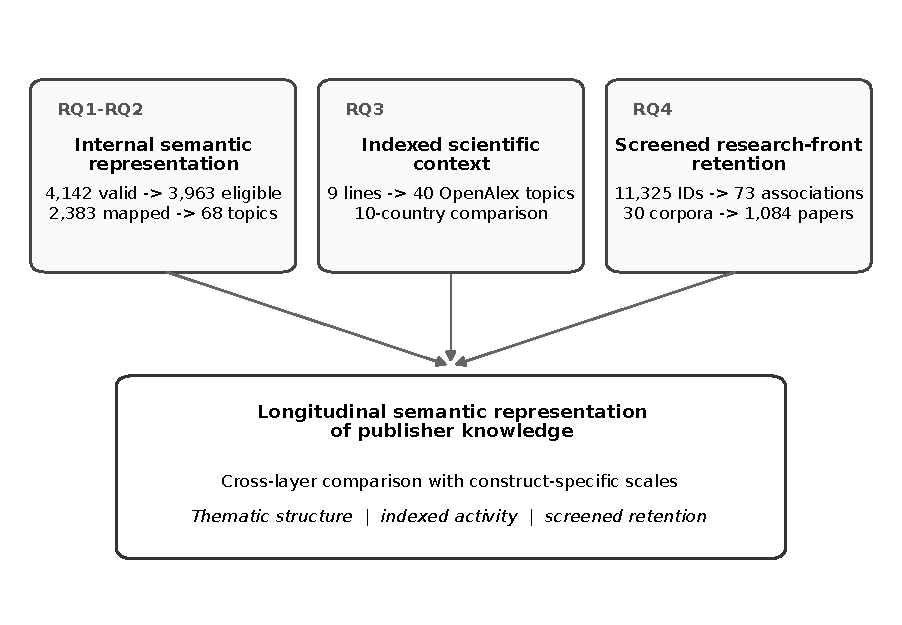
\includegraphics[width=\textwidth]{figures/Fig1_framework.pdf}
\caption{Analytical architecture of the proposed framework. The internal semantic representation, OpenAlex indexed-activity context, and screened Research Horizon retention form distinct evidence layers that are compared across the four research questions while retaining construct-specific scales.}\label{fig:framework}
\end{figure}

Table~\ref{tab:rqs} makes the research-question traceability explicit. This mapping is defined before the empirical results so that the evidence used to answer each question is clear.

\begin{table}[t]
\caption{Research questions, evidence layers, and analytical outputs}\label{tab:rqs}
\small
\begin{tabularx}{\textwidth}{@{}p{0.07\textwidth}Y Y Y@{}}
\toprule
RQ & Primary evidence & Methodological operation & Main results location \\
\midrule
RQ1 & Curated catalogue, longitudinal topic series & Semantic mapping; Hill diversity, concentration, persistence, continuity, compositional distance, and reference renewal classification & Sections~\ref{subsec:landscape}--\ref{subsec:profiles} \\
RQ2 & Initial algorithmic and curated topic states & Document-level curation diff; pre/post diversity and family comparison; hierarchy sensitivity & Sections~\ref{subsec:funnel}--\ref{subsec:landscape} \\
RQ3 & 40 unique OpenAlex topics mapped to nine editorial lines & Topic-country activity model; line-country aggregation; bounded territorial and weight sensitivity & Section~\ref{subsec:openalexres} \\
RQ4 & 11,325 Research Horizon topic IDs, 73 screened associations, 30 candidate corpora & Expert-assisted screening; corpus-wide documentary review; retained-candidate fraction and role composition & Sections~\ref{subsec:rhres}--\ref{subsec:integratedresults} \\
\bottomrule
\end{tabularx}
\end{table}

\section{Data and methods}\label{sec:methods}

\subsection{Study design and evidence layers}\label{subsec:design}

The study is a longitudinal methodological proof-of-concept. It reconstructs a publisher's internal thematic trajectory from frozen model-ready inputs and relates that trajectory to external indexed activity and screened research-front candidates through construct-specific evidence layers. The design contains four sequential evidence layers: (1) a source-flagged valid publisher catalogue; (2) an initial algorithmic semantic partition followed by documented expert curation; (3) longitudinal structural measures and a thematic-renewal classification; and (4) external mappings to OpenAlex and Research Horizon. Figure~\ref{fig:pipeline} shows the corpus-to-map sequence. Table~\ref{tab:sources} summarizes the full evidence design.

\begin{figure}[t]
\centering
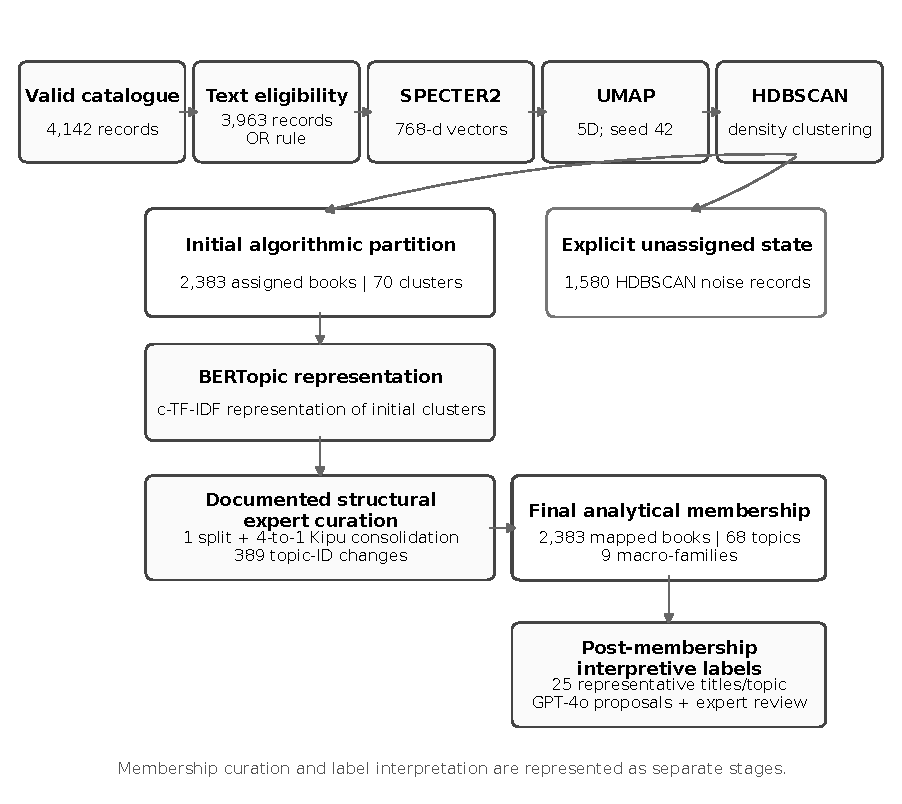
\includegraphics[width=\textwidth]{figures/Fig2_pipeline.pdf}
\caption{Corpus and semantic-mapping workflow. Initial algorithmic clustering, documented structural expert curation, final analytical membership, and post-membership labeling are represented as distinct stages; HDBSCAN noise remains explicitly unassigned in the reference semantic map.}\label{fig:pipeline}
\end{figure}

\begin{table}[t]
\caption{Evidence sources and their analytical role}\label{tab:sources}
\small
\begin{tabularx}{\textwidth}{@{}p{0.22\textwidth}p{0.25\textwidth}Y@{}}
\toprule
Source & Coverage used in this study & Analytical role \\
\midrule
Unified \ABYA\ book catalogue & 4,142 source-flagged valid book records, 1978--2026; cut-off 22 July 2026 & Internal longitudinal evidence; title/abstract semantic representation; book as unit of analysis \\
Reproducibility package & 3,963 semantically eligible records; SPECTER2 embeddings, anchored UMAP arrays, initial algorithmic and curated topic states & Algorithmic topic discovery, curation audit, hierarchy, annual topic series, reproducibility \\
OpenAlex & 40 unique topics, 46 editorial-line mappings, 10 pre-specified countries, 2015--2025 window & Comparative indexed scientific activity: accumulated/recent activity, world share, international collaboration, growth \\
Research Horizon & 11,325 topic IDs (11,232 unique names); 73 candidate associations; 30 Priority-1 datasets; 1,084 papers & Candidate research-front screening and corpus-wide documentary review \\
\bottomrule
\end{tabularx}
\end{table}

The internal representation combines semantic topic membership, hierarchical family context, longitudinal profile attributes, and documented curation provenance. Indexed scientific activity and research-front retention after documentary review are then attached to selected thematic units as separate contextual evidence. Each construct retains its original scale and interpretation.

\subsection{Catalogue, unit of analysis, and text eligibility}\label{subsec:corpus}

The source is the unified catalogue of books published by Editorial \ABYA. The upstream acquisition layer recorded 8,399 source rows and flagged 4,142 as valid book records. The frozen source record does not preserve the row-level reasons for all 4,257 upstream exclusions, so the 8,399-row figure is retained only as provenance and is not used as an analytical denominator. The unit of analysis throughout the internal layer is the source-flagged valid book record. The year variable is the editorial year available in the catalogue.

A record entered the semantic analysis if it satisfied at least one of two text-availability conditions: a title of at least 20 characters \emph{or} an abstract/summary of at least 200 characters. This canonical OR rule yielded 3,963 semantically eligible books and left 179 valid catalogue books outside the embedding-based analysis. For each eligible record, the model-ready input is the English-translated title followed, when available, by the English-translated abstract or summary; the reproducibility package preserves these exact strings together with the original titles. Translation occurred upstream in the analytical platform and is treated here as a fixed preprocessing input; it is not re-estimated in the reproducibility package. The semantic analysis therefore reproduces the model from frozen text inputs rather than auditing the translation procedure itself.

The temporal coverage begins in 1978, but the early years are sparse and the source contains no record for 1979. We therefore distinguish a 1978--1986 prelude from the effective long-run series beginning in 1987. The main interpretive periodization is 1987--1998 (foundation), 1999--2008 (diversified plateau), 2009--2014 (maximum expansion), 2015--2021 (contraction and transition), and 2022--2026 (recent recomposition). The 2025 and 2026 records reflect the latest catalogue update and are incomplete relative to earlier years; recent descriptive comparisons therefore give priority to the complete 2022--2024 observations. The Kipu documentary series receives a separate chronological treatment because its catalogue year tracks editorial registration and does not necessarily reproduce the original date of each underlying periodical item.

\subsection{Semantic representation and initial algorithmic topic discovery}\label{subsec:topicmodel}

Documents were represented with SPECTER2 (\texttt{allenai/specter2\_base}), producing a 768-dimensional vector for each semantically eligible book. SPECTER2 was developed for scientific document representation and evaluated across heterogeneous scientific tasks and fields \citep{singh2023scirepeval}. Its disciplinary breadth provides a practical reason for using it with a catalogue that spans social sciences, humanities, education, environmental studies, and technical fields. Its transfer from scientific documents to scholarly monographs is treated as a specific source of model uncertainty and is evaluated within the study's limitations.

The initial algorithmic topic model follows the BERTopic architecture \citep{grootendorst2022bertopic}. SPECTER2 embeddings were projected to five dimensions with UMAP \citep{mcinnes2018umap} and then clustered with HDBSCAN \citep{mcinnes2017hdbscan}. BERTopic used the resulting cluster memberships to construct class-based TF-IDF topic representations. A separate two-dimensional UMAP projection was retained only for visualization; it did not determine cluster membership. Table~\ref{tab:parameters} lists the fixed software versions and primary parameters.

\begin{table}[t]
\caption{Frozen topic-model configuration used in the reproducibility package}\label{tab:parameters}
\small
\begin{tabularx}{\textwidth}{@{}p{0.24\textwidth}p{0.27\textwidth}Y@{}}
\toprule
Component & Configuration & Role \\
\midrule
Environment & Python 3.11; BERTopic 0.16.4; UMAP 0.5.12; HDBSCAN 0.8.44; NumPy 1.26.4; scikit-learn 1.9.0 & Version-pinned analytical environment \\
Embedding & SPECTER2 base; 768 dimensions & Semantic document representation \\
UMAP for clustering & $n_{neighbors}=15$; $min\_dist=0.1$; cosine metric; 5 dimensions; random seed 42 & Nonlinear dimensionality reduction before density clustering \\
HDBSCAN & $min\_cluster\_size=10$; $min\_samples=None$; Euclidean metric; EOM cluster selection & Density-based cluster discovery with explicit noise \\
Topic representation & 1--2 grams; $min\_df=2$; English stopword set plus documented generic-term list; c-TF-IDF & Interpretable topic keywords after clustering \\
Visualization & 2D UMAP, seed 42 & Map coordinates only; not used to fit clusters \\
Label proposal & Top 25 representative titles; GPT-4o; expert review and renaming & Post-clustering interpretive label layer; membership fixed beforehand \\
\bottomrule
\end{tabularx}
\end{table}

The initial algorithmic solution is evaluated as a density-based partition with explicit noise. HDBSCAN assigns observations outside sufficiently dense semantic regions to $-1$, and the reference map retains those observations as unassigned. This decision prioritizes specificity of the stable thematic cores while preserving the outlier population for sensitivity analysis. Historical variation in metadata richness may contribute to non-assignment; the noise label is therefore interpreted as a density outcome rather than a data-quality category.

\subsection{Documented expert curation}\label{subsec:curation}

The initial algorithmic topic solution serves as the reference state for subsequent expert curation. Two kinds of curation were applied after clustering: structural operations on topic membership and interpretive operations on topic labels. The reproducibility package stores both the initial algorithmic state and the final curated state, together with a document-level diff, so the intervention and its consequences can be inspected directly.

Structural curation addressed two identifiable editorial situations. One broad initial cluster was split into two analytical lines, while four initial clusters corresponding to segments of the Kipu press/documentary series were consolidated into one documentary topic. The criteria were based on representative titles, semantic content, and known editorial-series provenance. The exact number of affected documents and the changes in global structure are reported in the Results because they are outcomes of applying the curation protocol, not method definitions.

Topic labels were generated after membership was defined. The pipeline used the 25 most representative titles per topic to propose labels with GPT-4o; experts then retained or renamed labels. The final state records whether each label is LLM-derived or manual. The LLM therefore assists interpretation after cluster membership has been fixed. This bounded role and the preservation of source evidence are consistent with recent calls for explicit evidence access and verification in LLM-supported scientometric workflows \citep{lee2026evidence}. The labels are used as a descriptive interpretive layer supported by preserved provenance. Independent retrospective double coding would provide an additional reliability assessment in subsequent validation work.

\subsection{Longitudinal structure and internal thematic profile}\label{subsec:longmetrics}

We characterize the catalogue at two levels: overall thematic composition and line-level trajectories. For each year or analysis period, let $n_{kt}$ be the number of mapped books assigned to topic $k$, $N_t=\sum_k n_{kt}$, and $p_{kt}=n_{kt}/N_t$. Three overall composition measures are used:

\begin{align}
HHI_t &= \sum_k p_{kt}^{2}, \\
{}^{1}D_t &= \exp\!\left(-\sum_k p_{kt}\ln p_{kt}\right), \\
{}^{2}D_t &= \frac{1}{HHI_t}, \\
d(t,t') &= 1-\frac{\mathbf{p}_t\cdot\mathbf{p}_{t'}}{\|\mathbf{p}_t\|\,\|\mathbf{p}_{t'}\|}.
\label{eq:composition}
\end{align}

$HHI_t$ measures concentration. ${}^{1}D_t$ is the Hill diversity of order 1 (the exponential of Shannon entropy), whereas ${}^{2}D_t=1/HHI_t$ is Hill diversity of order 2 \citep{shannon1948theory,hill1973diversity}. Reporting both orders prevents the Shannon-effective count from being read as the reciprocal of HHI. The cosine distance $d(t,t')$ measures compositional change between period vectors. All four quantities are interpreted specifically as properties of mapped thematic composition.

Two temporal schemes serve different analytical purposes. Six unequal interpretive periods (1978--1986, 1987--1998, 1999--2008, 2009--2014, 2015--2021, and 2022--2026) summarize historically meaningful phases of catalogue development. Compositional distance uses a separate sequence of adjacent, non-overlapping windows: the 1978--1986 prelude followed by five-year blocks from 1987--1991 through 2022--2026. The 2017--2021 to 2022--2026 comparison is therefore the final pair in this standardized distance series. The complete-year sensitivity check replaces the last block with 2022--2024.

For line-level analysis, five continuous dimensions summarize distinct aspects of internal thematic strength and are retained as a vector of construct-specific measures. Table~\ref{tab:internaldims} defines the components. For topic $k$, let $n_k$ denote total mapped books, $d_k$ the number of active decades among the five long-run decades, $a_k$ the number of active years, and $\ell_k=y^{last}_k-y^{first}_k+1$ the observed span. Let $R_k$ and $B_k$ denote topic-$k$ book counts in 2015--2026 and 2003--2014, respectively. Volume is relative topic size; persistence records how many of the five long-run decades contain activity; continuity measures the share of active years within the observed span; recent growth combines the minimum recent-volume threshold with the recent-to-previous ratio; and within-family prominence records the topic's volume relative to the largest topic in its macro-family. Each dimension is scaled to 0--100 to place heterogeneous quantities on a common display range. Interpretation remains dimension-specific, so equal numerical differences across dimensions carry the meaning of their respective operational definitions.

\begin{table}[t]
\caption{Continuous internal thematic-profile dimensions}\label{tab:internaldims}
\footnotesize
\setlength{\tabcolsep}{3.5pt}
\begin{tabularx}{\textwidth}{@{}p{0.16\textwidth}c p{0.39\textwidth}Y@{}}
\toprule
Dimension & Symbol & Operationalization & Interpretation \\
\midrule
Volume & $V$ & $100\,n_k/\max_j n_j$ & Relative catalogue accumulation \\
Persistence & $P$ & $100\,d_k/5$; $d_k$ = active decades & Long-run temporal presence \\
Continuity & $C$ & $100\,a_k/\ell_k$; active years / observed span & Regularity within the trajectory \\
Recent growth & $G$ & \makecell[l]{$100\min(R_k/10,1)$\\$\times\min((R_k/\max(B_k,1))/1.5,1)$} & Screening signal for subsequent renewal qualification \\
Within-family prominence & $F$ & $100\,n_k/\max_{j\in F(k)}n_j$ & Relative volume within the macro-family \\
\bottomrule
\end{tabularx}
\end{table}

The macro-families are obtained by cutting the BERTopic hierarchy at distance threshold 5.0. Sensitivity was checked around this cut: thresholds 4.0, 4.25, 4.5, 4.75, 5.0, 5.25, and 5.5 produce 12, 11, 10, 9, 9, 8, and 7 families, respectively. The nine-family solution is therefore locally stable over the 4.75--5.0 interval. Family membership is determined by the hierarchy, and the family names provide its interpretive labels.

\subsection{Two-stage classification of substantive recent renewal}\label{subsec:renewalmethod}

Substantive thematic renewal is operationalized through two sequential conditions: an algorithmic expansion signal followed by trajectory qualification. Let $R^{15\text{--}26}_k$ and $R^{03\text{--}14}_k$ denote topic-$k$ book counts in 2015--2026 and 2003--2014, respectively, and let $y^{first}_k$ and $y^{last}_k$ denote the first and last active years. The original workflow defined an emergent topic as one whose first active year is 2013 or later. Stage A flags an expansion candidate when

\begin{equation}
\mathrm{Expansion}_k = [R^{15\text{--}26}_k\ge 10]
\land \left[\frac{R^{15\text{--}26}_k}{\max(R^{03\text{--}14}_k,1)}\ge 1.5\right]
\land [y^{first}_k<2013].
\label{eq:stageA}
\end{equation}

The emergence exclusion affects two of the 68 final topics: \emph{Decolonial pedagogies and insurgent practices} (first active year 2013) and \emph{Yánkuam diaries in Peru and Ecuador} (2018). Both remain part of the thematic map and are excluded only from the expansion-versus-renewal classification because their observed trajectories begin within the recent-growth era.

Stage B was retrospectively formalized from exclusion reasons documented during the original analytical workflow. The resulting rule makes the recorded case decisions executable independently of topic names or IDs. General validity remains to be established through prespecified cross-publisher replication. Let $I^{time}_k$ equal 1 when no documented chronological anomaly compromises the series; let $q^{(3)}_k$ be the share of all topic-$k$ books concentrated in its three highest-output years; let $\ell_k=y^{last}_k-y^{first}_k+1$ be the observed span; and let $n_k$ be total mapped books in the topic. Episodicity is defined as

\begin{equation}
\mathrm{Episodic}_k=[q^{(3)}_k\ge0.60]\land[\ell_k\ge10]\land[n_k\ge15].
\label{eq:episodic}
\end{equation}

A reference substantive-renewal classification is then

\begin{equation}
\mathrm{Renewal}_k=\mathrm{Expansion}_k\land I^{time}_k
\land\neg\mathrm{Episodic}_k\land[y^{last}_k\ge2022].
\label{eq:stageB}
\end{equation}

The recency gate uses 2022 because 2022--2026 is the independently defined recent recomposition period. The chronological-integrity condition is evaluated upstream; after correction for the Kipu registration-date anomaly, the frozen Stage-A set contains eight candidates. Because Stage B was formalized ex post, the four-topic outcome is treated as the reference-case classification and its threshold dependence is evaluated explicitly. Sensitivity is evaluated over 36 combinations of the growth-ratio threshold (1.25, 1.50, 1.75), episodicity threshold (0.50, 0.55, 0.60, 0.65), and final-year gate (2021, 2022, 2023). These rules can be prespecified before candidate inspection in future replications.

\subsection{OpenAlex indexed scientific activity}\label{subsec:openalexmethod}

Nine editorial lines were selected for the external proof-of-concept: six lines with strong historical convergence in the internal catalogue and three additional lines identified through substantive recent renewal. Amazonian literature and culture is itself a renewed line but was already present in the historical block, so it does not increase the nine-line set. The nine lines were mapped to 46 line-topic correspondences involving 40 unique OpenAlex topics. Each correspondence was classified by its role in representing the editorial line: principal (weight 1.00), complementary (0.65), specific subline (0.55), or contextual/partial (0.35).

For each OpenAlex topic $o$ and country $c$, five signals were computed: production in 2015--2025, recent production in 2021--2025, world share, international collaboration, and growth trend. Signals were normalized within the ten pre-specified countries for each topic. The production component uses logarithmic transformation before normalization. The topic-country score has an effective maximum of 90 points:

\begin{equation}
Q_{oc}=30\tilde{N}^{15\text{--}25}_{oc}+25\tilde{N}^{21\text{--}25}_{oc}
+15\tilde{W}_{oc}+10\tilde{C}_{oc}+10\tilde{T}_{oc}.
\label{eq:openalex}
\end{equation}

A line-country score is the role-weighted mean of the mapped topic-country scores, rescaled once from 90 to 100,

\begin{equation}
A_{\ell c}=\frac{100}{90}\,
\frac{\sum_{o\in O_{\ell}} w_{\ell o}Q_{oc}}
{\sum_{o\in O_{\ell}}w_{\ell o}}.
\label{eq:linecountry}
\end{equation}

The ten-country comparison comprises Ecuador, Mexico, Spain, Colombia, Peru, Argentina, Bolivia, Brazil, Chile, and the United States. This set was pre-specified before the present comparative analysis and is retained as a bounded comparison set. Because OpenAlex coverage and metadata quality vary by language, field, and indexing infrastructure, country scores are conditional on database representation; evidence from Latin America suggests broader Spanish-language and SSH coverage than Scopus in some settings, while independent audits also identify language-metadata errors \citep{gallardo2024openalex,cespedes2025linguistic}. The equal-country comparison serves as the scientific reference scenario. A second, alternative strategic scenario weights Ecuador--Mexico--Spain at 60\% and the other seven countries at 40\% when a line-level territorial summary is needed. Robustness checks perturb the component and mapping-role weights and compare the strategic scenario with the equal-country territorial pattern.

\subsection{Research Horizon screening and documentary review}\label{subsec:rhmethod}

Clarivate Research Horizon Navigator serves as a fixed exported source of candidate emerging-topic clusters; research-front relevance is subsequently qualified through corpus-wide documentary review. The exported universe available to the study contained 11,325 topic IDs corresponding to 11,232 unique names. Candidate generation combined the nine internal editorial profiles, OpenAlex bridge topics, expanded textual retrieval, and manual review. This structured expert-assisted screening produced 73 line-cluster associations: 30 Priority 1, 16 Priority 2, and 27 Reserve. The screening files also preserve false-positive examples, which are important because lexical proximity alone sometimes retrieves clusters that are regionally or substantively unrelated to the editorial line.

A preliminary 100-point affinity heuristic supported prioritization of candidate datasets: thematic correspondence (45 points), bridge with OpenAlex (25), fit with the editorial line (20), and regional/cultural signal (10). The heuristic did not determine the final frontier category. All 30 Priority-1 datasets were obtained, comprising 1,084 paper records. The recorded dataset sizes match the consolidated record-level corpus exactly. Titles, abstracts, keywords, subject composition, affiliations, and representative papers were then reviewed to classify each candidate as principal, complementary, specific subline, reserve, or excluded.

For each editorial line $\ell$, the primary research-front output is the retained-candidate fraction

\begin{equation}
H_{\ell}=\frac{N^{principal}_{\ell}+N^{complementary}_{\ell}+N^{specific}_{\ell}}{N^{reviewed}_{\ell}},
\label{eq:rhretention}
\end{equation}

reported together with the role composition of retained candidates. The numerator includes principal, complementary, and specific-subline candidates, while reserve and excluded cases remain outside the retained set. $H_{\ell}$ is interpreted as a bounded survival fraction within the Priority-1 set screened for each line, whose denominator ranges from two to six. It therefore answers the question ``what share of the screened candidate set survived documentary review?'' while keeping the line-specific screening intensity visible in the denominator.

The screening provides a traceable path from the 11,325-topic exported universe through candidate associations to the 30 Priority-1 corpora and their final documentary review of the available paper records. Its empirical scope is the recorded candidate funnel rather than exhaustive retrieval of every potentially relevant topic. The original candidate classification was conducted by one expert; independent retrospective double coding is therefore identified as a subsequent validation step.

\subsection{Reproducibility, robustness, and evaluation strategy}\label{subsec:robustnessmethod}

Reproducibility is handled differently for deterministic and interpretive components. The topic-model package contains the 3,963 model records, frozen model inputs, 768-dimensional embeddings, original five- and two-dimensional UMAP arrays, initial algorithmic reference clusters, final curated state, parameter files, a version-pinned environment, hashes, notebooks, and verification scripts. Starting from the anchored five-dimensional UMAP representation, the frozen clustering state can be checked against the stored assignments. UMAP re-projection from embeddings uses a fixed seed but can still vary slightly across software and numerical environments; the archived arrays therefore define the hard computational reference. LLM-generated labels and expert decisions are frozen provenance data rather than deterministic model output. This distinction follows the broader principle that multi-step bibliometric workflows should expose both computational operations and input dependencies \citep{guler2016workflows,lee2026evidence}. All quantitative values reported here derive from executed scripts over frozen data and preserved analytical states. The computational and interpretive stages are therefore distinguished by their provenance and reproducibility characteristics.

The robustness design targets the main analytical decisions. First, initial algorithmic and curated thematic states are compared directly. Second, the macro-family cut is varied around the selected threshold. Third, assignment rates and simple preserved-text characteristics are compared for assigned and unassigned records. Fourth, outlier sensitivity is examined in two ways using the frozen SPECTER2 embeddings. An intentionally aggressive stress test assigns every HDBSCAN noise record to its nearest final-topic cosine centroid. A controlled high-confidence scenario reassigns only noise records that exceed the 25th-percentile thresholds of both own-topic centroid similarity and assignment margin observed among mapped records. The reference map remains the primary specification, while these scenarios quantify the dependence of downstream diversity, compositional distance, and renewal membership on the outlier policy. Fifth, the two-stage renewal rule is perturbed over 36 threshold combinations. Sixth, the 2017--2021 to 2022--2026 compositional change is recomputed using the complete 2022--2024 subwindow. Seventh, HDBSCAN minimum-cluster-size sensitivity is explored on the archived five-dimensional representation using a cross-implementation perturbation; the reference-like setting is first checked against the frozen initial algorithmic partition with ARI and NMI. The frozen execution environment does not support an exact historical UMAP $n\_neighbors$ rerun, so neighborhood coherence is inspected at 10, 15, 20, and 30 nearest neighbors in the original 768-dimensional embedding space. This provides a semantic-neighborhood-scale diagnostic that is analytically distinct from a UMAP-parameter sensitivity test. Finally, the OpenAlex geographic conclusions are compared under equal-country and 60/40 territorial scenarios and under 5,000 Monte Carlo perturbations of component and mapping-role weights. The original interpretive classifications were produced by one expert and retain frozen provenance; a separate retrospective double-coding exercise on the preserved corpora would provide additional inter-rater validation. Detailed results of these robustness checks are reported in Appendix~\ref{app:robustness}; the accompanying reproducibility package is summarized in the Data Availability Statement.

\section{Results: longitudinal proof-of-concept}\label{sec:results}

The proof-of-concept is reported in the same sequence as the analytical framework: first the coverage and stability of the internal thematic map, then long-run thematic change, the multidimensional profiles of the nine focal lines, indexed scientific activity, and finally research-front retention. Results from the three evidence layers are kept separate throughout this section. Their joint interpretation is reserved for Section~\ref{subsec:integratedresults} and the Discussion.

\subsection{Corpus coverage and the effect of documented curation}\label{subsec:funnel}

The catalogue contained 4,142 valid book records after upstream consolidation. The text-eligibility rule retained 3,963 records for semantic modelling; 179 valid books did not meet either the title-length or abstract-length condition. HDBSCAN assigned 2,383 of the semantically eligible books to stable density regions and left 1,580 as noise. The resulting assignment rate is 60.1\% among semantically eligible books and 57.5\% relative to the full valid catalogue. These percentages define the evidential scope of all topic-level results below: the thematic map describes the stable semantic cores identified by the model, not every valid book in the catalogue.

The non-assigned share is substantial, but it is not concentrated in a single historical decade. Among semantically eligible records, assignment rates were 65.2\% in 1978--1989, 64.0\% in the 1990s, 59.7\% in the 2000s, 58.2\% in the 2010s, and 59.2\% in 2020--2026. The decline from the earliest periods is moderate rather than discontinuous. This pattern is consistent with the interpretation of HDBSCAN noise as the complement of stable density regions, while also leaving open the possibility that historical differences in metadata richness affect assignment probabilities.

\begin{table}[t]
\caption{Corpus funnel and semantic assignment coverage}\label{tab:funnel}
\small
\begin{tabularx}{\textwidth}{@{}YrrY@{}}
\toprule
Stage & Records & Share & Interpretation \\
\midrule
Valid consolidated catalogue & 4,142 & 100.0\% of valid books & Documentary universe used for descriptive counts \\
Semantically eligible & 3,963 & 95.7\% of valid books & Title $\geq20$ characters OR abstract $\geq200$ characters \\
Assigned to stable topics & 2,383 & 60.1\% of eligible books & Basis of topic, family, continuity, and composition analyses \\
HDBSCAN noise & 1,580 & 39.9\% of eligible books & Retained as unassigned; no nearest-topic forcing \\
Outside semantic eligibility & 179 & 4.3\% of valid books & Remain part of the valid catalogue but not of the semantic model \\
\bottomrule
\end{tabularx}
\end{table}

The initial algorithmic partition contained 70 clusters before expert curation. The documented structural curation produced 68 final analytical topics while preserving the same 2,383 assigned books. A document-level comparison between the two states identifies 389 records whose topic identifier changed, equivalent to 9.82\% of the 3,963 semantically eligible records. The intervention therefore affected a bounded subset rather than replacing the initial algorithmic structure wholesale. It also changed the global distribution modestly: concentration decreased from $HHI=0.0316$ in the initial algorithmic solution to $0.0259$ in the curated map, while Hill diversity of order 1 increased from 49.83 to 51.10. In the curated map, Hill diversity of order 2 is 38.60. These changes follow from splitting a broad mixed cluster and consolidating the four Kipu segments into a documentary-series topic.

\begin{table}[t]
\caption{Initial algorithmic and expert-curated thematic states}\label{tab:auto_curated}
\small
\begin{tabularx}{\textwidth}{@{}YrrY@{}}
\toprule
Measure & Initial algorithmic state & Final curated state & Reading \\
\midrule
Topics/clusters & 70 & 68 & One broad cluster split; four Kipu clusters merged into one documentary topic \\
Assigned books & 2,383 & 2,383 & Curation changes organization, not the assigned-book denominator \\
Documents with changed topic identifier & -- & 389 & 9.82\% of semantically eligible records \\
Herfindahl concentration & 0.0316 & 0.0259 & Final map is slightly less concentrated \\
Hill diversity ${}^{1}D$ & 49.83 & 51.10 & Shannon-effective topic diversity increases slightly \\
\bottomrule
\end{tabularx}
\end{table}

This comparison answers RQ2 by quantifying the role of curation instead of treating expert intervention as an undocumented correction. The initial algorithmic partition and the expert-curated state remain separately inspectable.

The outlier-reassignment stress tests quantify how the 39.9\% noise share affects downstream results. Forcing all 1,580 noise records to the nearest final-topic centroid changes HHI from 0.0259 to 0.0242, Hill diversity ${}^{1}D$ from 51.10 to 53.01, and ${}^{2}D$ from 38.60 to 41.33. The global diversity structure is therefore comparatively stable. Temporal conclusions are more sensitive: the 2017--2021 to 2022--2026 cosine distance falls from 0.363 to 0.258 under complete forcing. A controlled high-confidence scenario reassigns only 166 noise records and yields ${}^{1}D=51.34$, ${}^{2}D=39.08$, and a recent distance of 0.334. Thus, the evidence supports a recent compositional shift across scenarios, but its magnitude depends on whether diffuse records are forced into stable topics.

The preserved fields do not support a complete diagnosis of why records became noise, but they do rule out one simple explanation. Unassigned records do not have shorter titles: the median original-title length is 66 characters among noise records versus 60 among assigned records; the corresponding model-text medians are 64 and 59. Exact duplicate-title shares are also similar (12.9\% vs. 12.5\%). Original-language and complete series metadata were not preserved at sufficient resolution for a comparable language-by-series characterization. The initial algorithmic partition remains observable, the exact modified documents are known, and the direction of the main diversity statistics can be checked before and after curation.

\subsection{The final thematic landscape: distributed concentration and long persistence}\label{subsec:landscape}

The final map contains 68 topics organized into nine hierarchical macro-families. Figure~\ref{fig:thematicmap} displays the 2,383 mapped books in the two-dimensional UMAP visualization, with topic centroids superimposed and the nine focal lines labelled. The two-dimensional coordinates are used only for visualization; topic membership derives from the five-dimensional clustering representation described in Section~\ref{subsec:topicmodel}.

\begin{figure}[t]
\centering
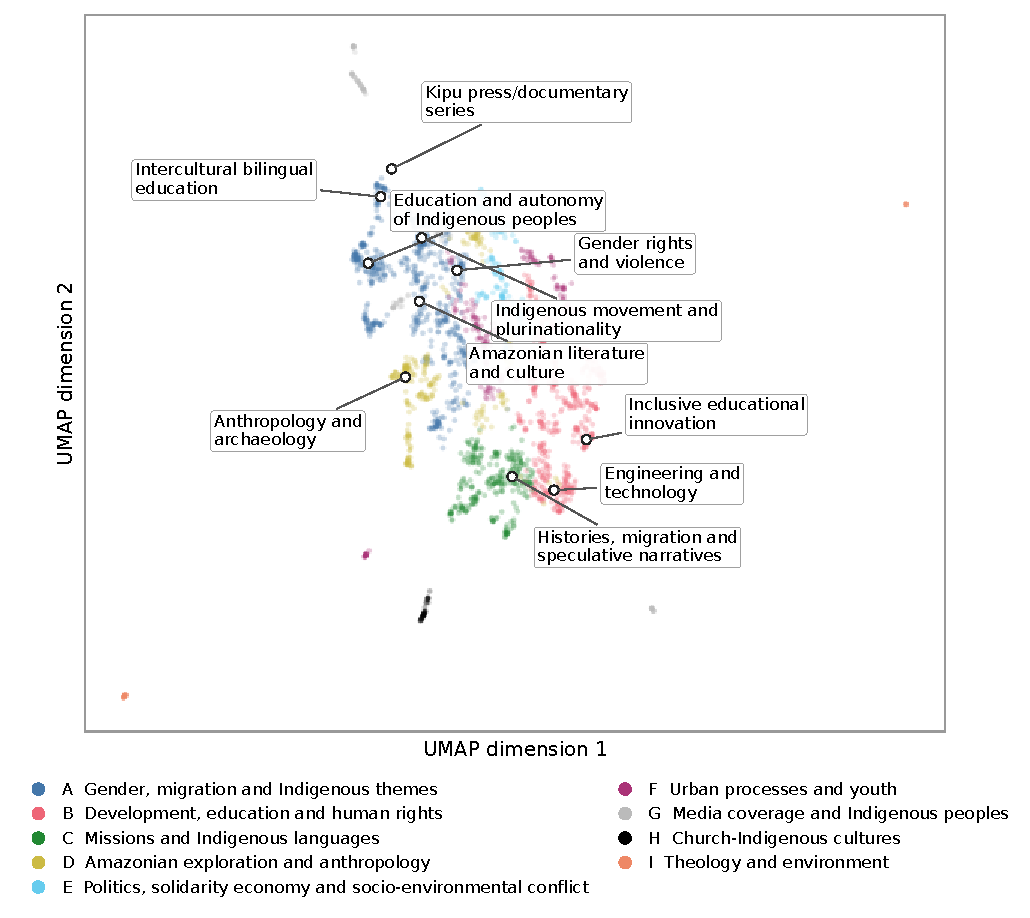
\includegraphics[width=\textwidth]{figures/Fig3_thematic_map.pdf}
\caption{General thematic map of the final curated catalogue. Each point is a book assigned to one of 68 analytical topics; colours identify the nine macro-families produced by the hierarchical cut. Only the centroids of the nine focal lines and the Kipu documentary series are marked and labelled. The two-dimensional UMAP layout is used for visualization; cluster membership derives from the five-dimensional clustering representation.}\label{fig:thematicmap}
\end{figure}

The topic-size distribution is broad rather than dominated by a few clusters. The final $HHI$ of 0.0259 corresponds to 51.10 effective topics, meaning that the observed concentration is comparable to a hypothetical distribution with about 51 equally common topics. The largest topic, \emph{Education and autonomy of Indigenous peoples}, contains 150 books (6.29\% of mapped books), followed by \emph{Engineering and technology} with 147 (6.17\%) and \emph{Histories, migration and speculative narratives} with 137 (5.75\%). The five largest topics together account for 26.5\% of the mapped corpus, leaving nearly three quarters distributed across the remaining 63 topics.

Long persistence is nevertheless widespread. Forty-six topics are active in at least four decades and together contain 1,952 books, or 81.9\% of mapped records. Eighteen topics appear in all five long-run decades used for the persistence calculation and account for 1,157 books (48.6\%). Persistence should not be read as uniform annual continuity: for example, \emph{Education and autonomy of Indigenous peoples} is active in 35 of the 37 years between its first and last mapped records, whereas \emph{Amazonian literature and culture} is active in 27 of 38 years. These distinctions motivate retaining persistence and continuity as separate profile dimensions.

\begin{table}[t]
\caption{Largest final topics and their longitudinal characteristics}\label{tab:largesttopics}
\small
\setlength{\tabcolsep}{4pt}
\begin{tabularx}{\textwidth}{@{}Yrrcrr@{}}
\toprule
Topic & Books & Share & Observed span & Active years & Active decades \\
\midrule
Education and autonomy of Indigenous peoples & 150 & 6.29\% & 1987--2023 & 35 & 5 \\
Engineering and technology & 147 & 6.17\% & 1987--2024 & 32 & 5 \\
Histories, migration and speculative narratives & 137 & 5.75\% & 1978--2025 & 38 & 5 \\
Kipu press/documentary series & 105 & 4.41\% & 1983--2024 & 40 & 5 \\
Indigenous movement and plurinationality & 92 & 3.86\% & 1989--2026 & 33 & 5 \\
Anthropology and archaeology & 76 & 3.19\% & 1988--2026 & 28 & 5 \\
Amazonian literature and culture & 65 & 2.73\% & 1987--2024 & 27 & 5 \\
Interculturality and cultural educational management & 61 & 2.56\% & 1989--2025 & 25 & 5 \\
Political culture and democracy & 60 & 2.52\% & 1989--2025 & 26 & 5 \\
Community development and university extension & 56 & 2.35\% & 2007--2023 & 14 & 3 \\
\bottomrule
\end{tabularx}
\end{table}

The nine macro-families are an interpretive higher-order organization rather than a substitute for the 68-topic map. Their sizes range from 681 mapped books in the largest family to 26 in the smallest. Varying the hierarchy cut confirms that the nine-family solution is locally stable but not uniquely determined: the number of families changes from 12 at threshold 4.0 to seven at 5.5, remaining at nine for thresholds 4.75 and 5.0. We therefore use the family layer to provide relational context and to calculate within-family prominence, not to claim a uniquely true taxonomy of the catalogue.

\subsection{Longitudinal evolution: historical accumulation and recent recomposition}\label{subsec:temporal}

The catalogue grows unevenly over the observation period. Figure~\ref{fig:longitudinal} combines annual catalogue and mapped-book counts with the separate sequence of adjacent, non-overlapping windows used for compositional distance; the incomplete 2025--2026 tail is marked explicitly. The 1978--1986 prelude contains only 17 valid books and 13 mapped books. Volume subsequently expands: 1987--1998 contains 870 valid and 513 mapped books; 1999--2008 contains 1,001 valid and 551 mapped books; and 2009--2014 reaches the maximum six-year volume with 1,073 valid and 612 mapped books. The annual valid-book count peaks at 242 in 2013. The following windows contain 844 valid and 488 mapped books in 2015--2021 and 337 valid and 206 mapped books in 2022--2026. The last window includes partial 2025--2026 catalogue coverage and is therefore interpreted primarily as a composition signal rather than a finalized volume estimate.

\begin{figure}[t]
\centering
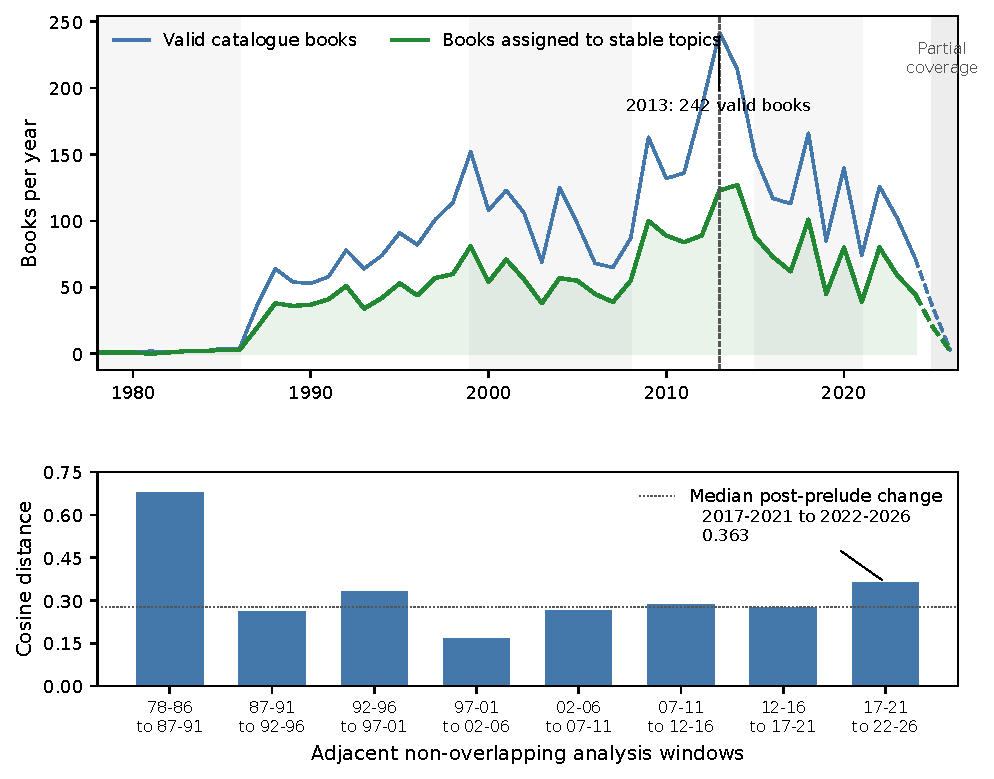
\includegraphics[width=\textwidth]{figures/Fig4_longitudinal.pdf}
\caption{Longitudinal catalogue volume and compositional change. The upper panel distinguishes annual valid catalogue books from books assigned to stable topics and marks 2025--2026 as partial catalogue coverage. The lower panel reports cosine distance between adjacent, non-overlapping analysis windows: the 1978--1986 prelude followed by five-year blocks. The 2017--2021 to 2022--2026 transition has a distance of 0.363; the complete 2022--2024 check yields 0.371.}\label{fig:longitudinal}
\end{figure}

\begin{table}[t]
\caption{Catalogue volume and mapped books by analytical period}\label{tab:periods}
\small
\begin{tabularx}{\textwidth}{@{}YrrrY@{}}
\toprule
Period & Valid books & Mapped books & Mapped / valid & Analytical reading \\
\midrule
1978--1986 & 17 & 13 & 76.5\% & Documentary prelude; too small for fine trend inference \\
1987--1998 & 870 & 513 & 59.0\% & Foundation and consolidation of long-run lines \\
1999--2008 & 1,001 & 551 & 55.0\% & Diversified plateau \\
2009--2014 & 1,073 & 612 & 57.0\% & Maximum catalogue expansion \\
2015--2021 & 844 & 488 & 57.8\% & Contraction and transition \\
2022--2026 & 337 & 206 & 61.1\% & Recent recomposition; 2025--2026 coverage is partial \\
\bottomrule
\end{tabularx}
\end{table}

Compositional change varies independently of total output. The transition from the small prelude to 1987--1991 has the largest raw distance (0.679), as expected from the very small initial base. Excluding that discontinuity, the 2017--2021 to 2022--2026 transition has the largest adjacent-window distance, 0.363. Earlier post-foundation distances range from 0.168 to 0.333. Restricting the recent window to the complete 2022--2024 years yields a slightly larger distance of 0.371, so incomplete 2025--2026 coverage does not account for the recent shift. Under the controlled high-confidence outlier reassignment, the corresponding distances are 0.334 and 0.341. The recent catalogue therefore differs in composition from the 2010s portfolio, although the magnitude of recomposition depends on how diffuse records are treated. The direction of change is selective rather than wholesale because many large historical topics remain active while a limited group of smaller lines increases its recent share.

This pattern provides the first answer to RQ1. Long-run thematic structure is characterized simultaneously by high persistence, distributed topic diversity, and episodic changes in composition, which are captured by separate longitudinal statistics.

\subsection{Internal thematic profiles and the distinction between growth and substantive renewal}\label{subsec:profiles}

Figure~\ref{fig:profiles} compares the five continuous internal dimensions across the nine focal editorial lines. Historically accumulated lines have different internal signatures. \emph{Education and Indigenous autonomy} combines maximum relative volume and persistence with 94.6 on continuity and within-family prominence of 100. \emph{Engineering and technology} is nearly as large (98.1 on relative volume) and persists across all five decades, but its recent-growth signal is only 32.5 because its 2015--2026 output is lower relative to the 2003--2014 base. \emph{Histories, migration and speculative narratives} also combines high volume and long persistence, while its continuity is lower than that of the education line.

\begin{figure}[t]
\centering
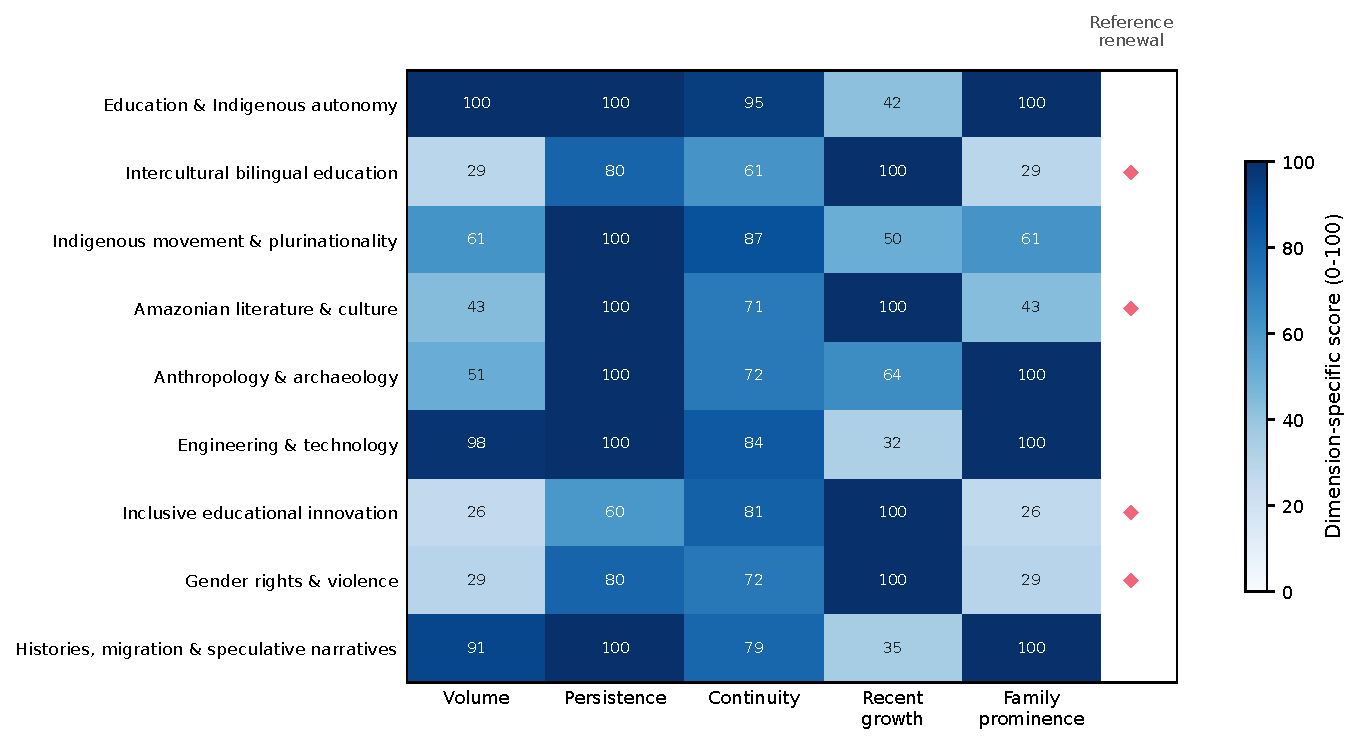
\includegraphics[width=\textwidth]{figures/Fig5_internal_profiles.pdf}
\caption{Five-dimensional internal thematic profiles for the nine focal editorial lines. Components use the 0--100 display scaling defined in Table~\ref{tab:internaldims}; each column retains its own operational meaning and is interpreted dimension by dimension. Diamonds identify lines that independently satisfy the reference two-stage substantive-renewal rule.}\label{fig:profiles}
\end{figure}

The three lines added to the external analysis because of renewal have a contrasting profile. \emph{Inclusive educational innovation} has a relative volume of 26.1 and persistence of 60, but continuity of 81.2 and the maximum recent-growth signal. \emph{Gender rights and violence} and \emph{Intercultural bilingual education} also have modest accumulated volume but maximum recent-growth scores. Amazonian literature and culture is the fourth renewed line; it was already included among the historically relevant lines and therefore does not add a tenth focal line. The profiles show that a relatively small stock can coexist with a strong current trajectory, while a very large historical stock can coexist with weaker recent growth.

\begin{table}[t]
\caption{Internal profile of the nine focal editorial lines}\label{tab:profiles}
\small
\begin{tabularx}{\textwidth}{@{}Yrrrrrrr@{}}
\toprule
Line & Books & $V$ & $P$ & $C$ & $G$ & $F$ & Renewal \\
\midrule
Education and Indigenous autonomy & 150 & 100.0 & 100 & 94.6 & 41.7 & 100.0 & No \\
Intercultural bilingual education & 43 & 28.6 & 80 & 61.1 & 100.0 & 28.7 & Yes \\
Indigenous movement and plurinationality & 92 & 61.4 & 100 & 86.8 & 50.0 & 61.3 & No \\
Amazonian literature and culture & 65 & 43.4 & 100 & 71.1 & 100.0 & 43.3 & Yes \\
Anthropology and archaeology & 76 & 50.7 & 100 & 71.8 & 64.3 & 100.0 & No \\
Engineering and technology & 147 & 98.1 & 100 & 84.2 & 32.5 & 100.0 & No \\
Inclusive educational innovation & 39 & 26.1 & 60 & 81.2 & 100.0 & 26.5 & Yes \\
Gender rights and violence & 44 & 29.4 & 80 & 71.9 & 100.0 & 29.3 & Yes \\
Histories, migration and speculative narratives & 137 & 91.4 & 100 & 79.2 & 34.9 & 100.0 & No \\
\bottomrule
\end{tabularx}
\end{table}

Two final topics are classified as emergent under the first-active-year cutoff: \emph{Decolonial pedagogies and insurgent practices} (2013) and \emph{Yánkuam diaries in Peru and Ecuador} (2018). They remain in the thematic map and are handled separately from the expansion screen. Stage A of the renewal procedure identifies eight expansion candidates among the non-emergent topics, and Stage B reduces these to four through topic-independent decision rules. Figure~\ref{fig:renewal} makes the logic visible. Three candidates---urban social inclusion, digital media and social networks, and citizen/multidimensional communication---have large recent-to-previous ratios but concentrate at least 60\% of their output in only three years, satisfying the pre-existing episodicity rule. Socio-environmental mining conflicts is not episodic, but its last mapped book is from 2020 and it therefore fails the 2022 recency gate. The four surviving lines are Amazonian literature and culture (38 vs. 13 books, ratio 2.92), inclusive educational innovation (27 vs. 12, ratio 2.25), intercultural bilingual education (19 vs. 12, ratio 1.58), and gender rights and violence (24 vs. 16, ratio 1.50).

\begin{figure}[t]
\centering
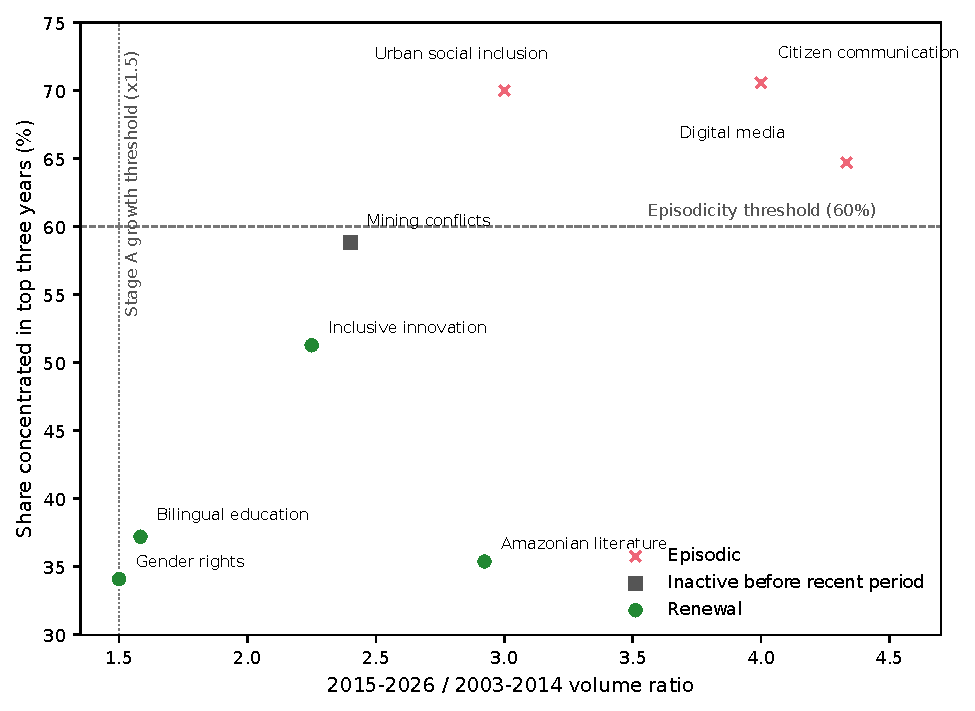
\includegraphics[width=\textwidth]{figures/Fig6_renewal.pdf}
\caption{Two-stage renewal classification for the eight current expansion candidates. The horizontal dashed line marks the 60\% top-three-year concentration threshold used by the episodicity rule; the vertical line marks the Stage-A growth-ratio threshold. The mining-conflict topic is non-episodic but is excluded because its last active year is 2020.}\label{fig:renewal}
\end{figure}

\begin{table}[t]
\caption{Audit trail for substantive recent renewal}\label{tab:renewal}
\small
\begin{tabularx}{\textwidth}{@{}YrrrrY@{}}
\toprule
Candidate & 2015--2026 & 2003--2014 & Ratio & Top-3-year share & Stage-B outcome \\
\midrule
Amazonian literature and culture & 38 & 13 & 2.92 & 35.4\% & Renewal; active to 2024 \\
Gender rights and violence & 24 & 16 & 1.50 & 34.1\% & Renewal; active to 2025 \\
Intercultural bilingual education & 19 & 12 & 1.58 & 37.2\% & Renewal; active to 2025 \\
Inclusive educational innovation & 27 & 12 & 2.25 & 51.3\% & Renewal; active to 2024 \\
Urban social inclusion & 15 & 5 & 3.00 & 70.0\% & Excluded as episodic \\
Digital media and social networks & 13 & 3 & 4.33 & 64.7\% & Excluded as episodic \\
Citizen and multidimensional communication & 12 & 3 & 4.00 & 70.6\% & Excluded as episodic \\
Socio-environmental mining conflicts & 12 & 5 & 2.40 & 58.8\% & Excluded; last active year 2020 \\
\bottomrule
\end{tabularx}
\end{table}

The comparison resolves a potential ambiguity in the term ``expansion.'' A fourfold increase is not necessarily substantive renewal when production is highly concentrated in a few years. Conversely, a ratio of 1.50 can qualify under the reference rule when the trajectory is non-episodic and remains active in the recent recomposition period. The four reference renewals are preserved under the controlled high-confidence outlier reassignment, but Stage-B threshold perturbation shows that exact membership is not invariant. Across 36 combinations of the growth-ratio threshold (1.25--1.75), episodicity threshold (50--65\%), and final-year gate (2021--2023), the number of renewals ranges from one to seven. Amazonian literature and culture is retained in all scenarios, inclusive educational innovation in 75.0\%, and gender rights and intercultural bilingual education in 66.7\% each. RQ1 is therefore answered by an executable reference classification whose general validity can be tested through prespecified cross-publisher replication.

\subsection{Indexed scientific activity across focal lines and countries}\label{subsec:openalexres}

OpenAlex produces a different view because the unit of comparison is scientific activity around mapped topics rather than books in the \ABYA catalogue. Figure~\ref{fig:openalex} reports the 90 line-country scores. Averaged over the nine lines, the United States has the highest comparative score among the ten pre-specified countries (71.47), followed by Spain (53.74), Brazil (52.36), Mexico (42.94), Argentina (36.99), and Chile (36.41). Ecuador's mean is 23.51 and Bolivia's 9.06. These values describe the relative configuration of the selected OpenAlex topics within this bounded ten-country comparison.

\begin{figure}[t]
\centering
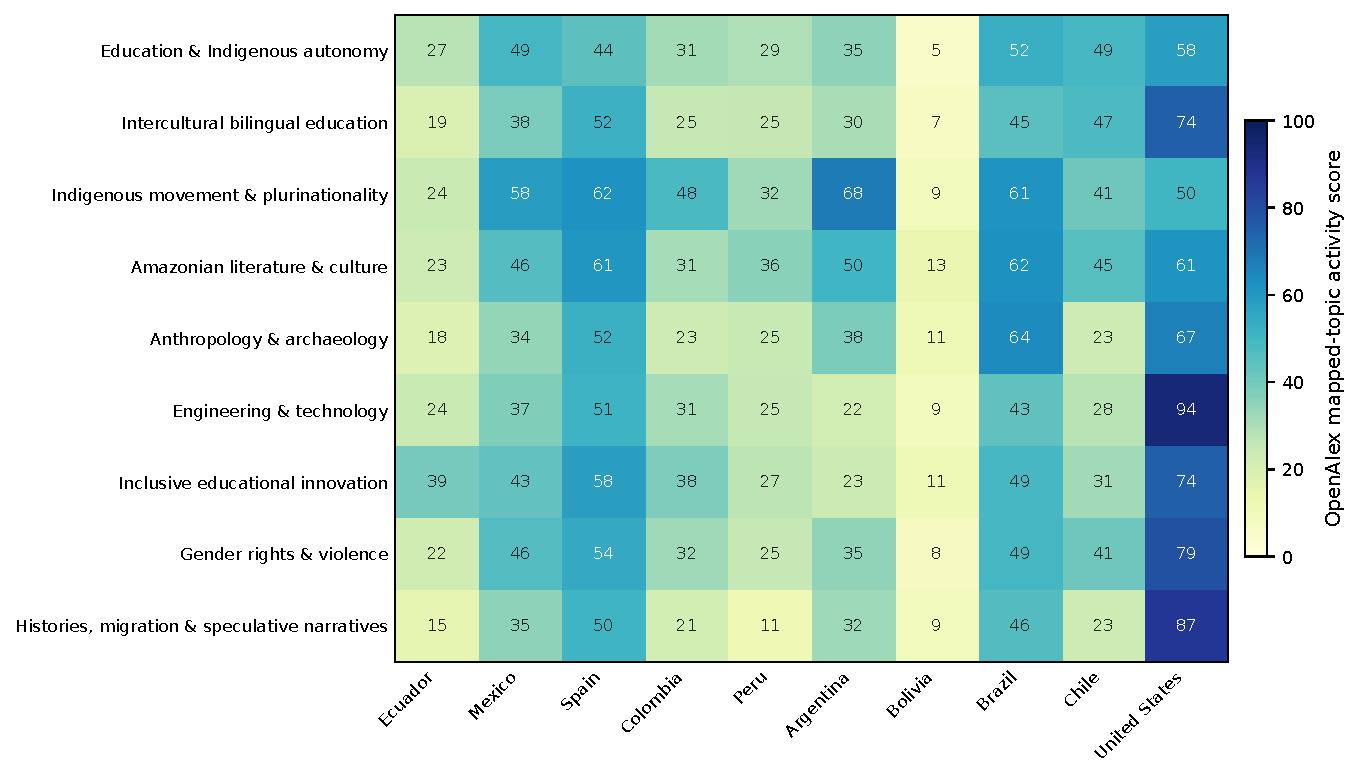
\includegraphics[width=\textwidth]{figures/Fig7_openalex_heatmap.pdf}
\caption{OpenAlex indexed scientific activity for the nine focal editorial lines across ten pre-specified countries. Cells report the line-country comparative score derived from mapped OpenAlex topics. The score is a comparative measure of indexed activity conditional on the selected topics, countries, period, and normalization procedure; its measurement scope is the bounded design used here.}\label{fig:openalex}
\end{figure}

The geography varies by editorial line. The United States has the highest score for seven of the nine lines, including engineering and technology (93.62), histories and migration (86.63), gender rights and violence (78.80), intercultural bilingual education (74.32), and inclusive educational innovation (74.43). Two lines differ. Argentina leads Indigenous movement and plurinationality with 67.88, ahead of Spain (61.72) and Brazil (61.08). Brazil leads Amazonian literature and culture with 62.14, narrowly ahead of the United States (60.97) and Spain (60.84). The result therefore supports a topic-by-territory reading rather than a single geographical hierarchy.

\begin{table}[t]
\caption{Highest OpenAlex line-country mapped-topic activity scores within the ten-country comparison}\label{tab:openalex_top}
\small
\begin{tabularx}{\textwidth}{@{}Yp{0.22\textwidth}rp{0.22\textwidth}r@{}}
\toprule
Editorial line & Highest country & Score & Second country & Score \\
\midrule
Education and Indigenous autonomy & United States & 58.09 & Brazil & 52.12 \\
Intercultural bilingual education & United States & 74.32 & Spain & 51.51 \\
Indigenous movement and plurinationality & Argentina & 67.88 & Spain & 61.72 \\
Amazonian literature and culture & Brazil & 62.14 & United States & 60.97 \\
Anthropology and archaeology & United States & 66.52 & Brazil & 63.72 \\
Engineering and technology & United States & 93.62 & Spain & 50.99 \\
Inclusive educational innovation & United States & 74.43 & Spain & 58.09 \\
Gender rights and violence & United States & 78.80 & Spain & 53.99 \\
Histories, migration and speculative narratives & United States & 86.63 & Spain & 50.46 \\
\bottomrule
\end{tabularx}
\end{table}

The strategic 60/40 territorial scenario does not materially reorder the nine lines relative to a simple equal-country mean. The Spearman rank correlation between the two line-level summaries is $\rho=0.983$, and the largest absolute score change is 3.21 points, for inclusive educational innovation. A separate 5,000-run perturbation of component and mapping-role weights leaves the United States first in the overall ten-country portfolio in every run; Spain and Brazil occupy second or third place in all simulations. These checks do not eliminate dependence on the chosen country set, but they show that the main comparative pattern is not a consequence of a single set of numerical weights.

These findings answer RQ3 within the scope of the pre-specified comparison. Indexed scientific activity around the mapped editorial themes varies substantially by topic and country, and the strongest country-level score depends on the theme. The ten-country set is a bounded, pre-specified comparison rather than a global sample, and OpenAlex coverage is itself heterogeneous. Evidence from Argentina indicates that OpenAlex can recover substantially broader Spanish-language and SSH production than Scopus \citep{gallardo2024openalex}, while a separate audit shows that OpenAlex language metadata can overestimate English and underestimate other languages \citep{cespedes2025linguistic}. The layer therefore provides bounded context on indexed scientific activity around mapped topics; direct impact of \ABYA books would require publication-level linkage evidence.

\subsection{Research-front retention after corpus-wide documentary review}\label{subsec:rhres}

The Research Horizon layer further separates preliminary metadata affinity from document-supported retention. Structured screening produced 30 Priority-1 candidate clusters whose corpora contained 1,084 paper records. Corpus-wide documentary review of titles, abstracts, keywords, subject fields, affiliations, and representative papers retained 23 clusters as principal, complementary, or specific sublines; four were placed in reserve and three were excluded. Across the 23 retained clusters, seven are principal, six complementary, and ten specific sublines.

\begin{figure}[t]
\centering
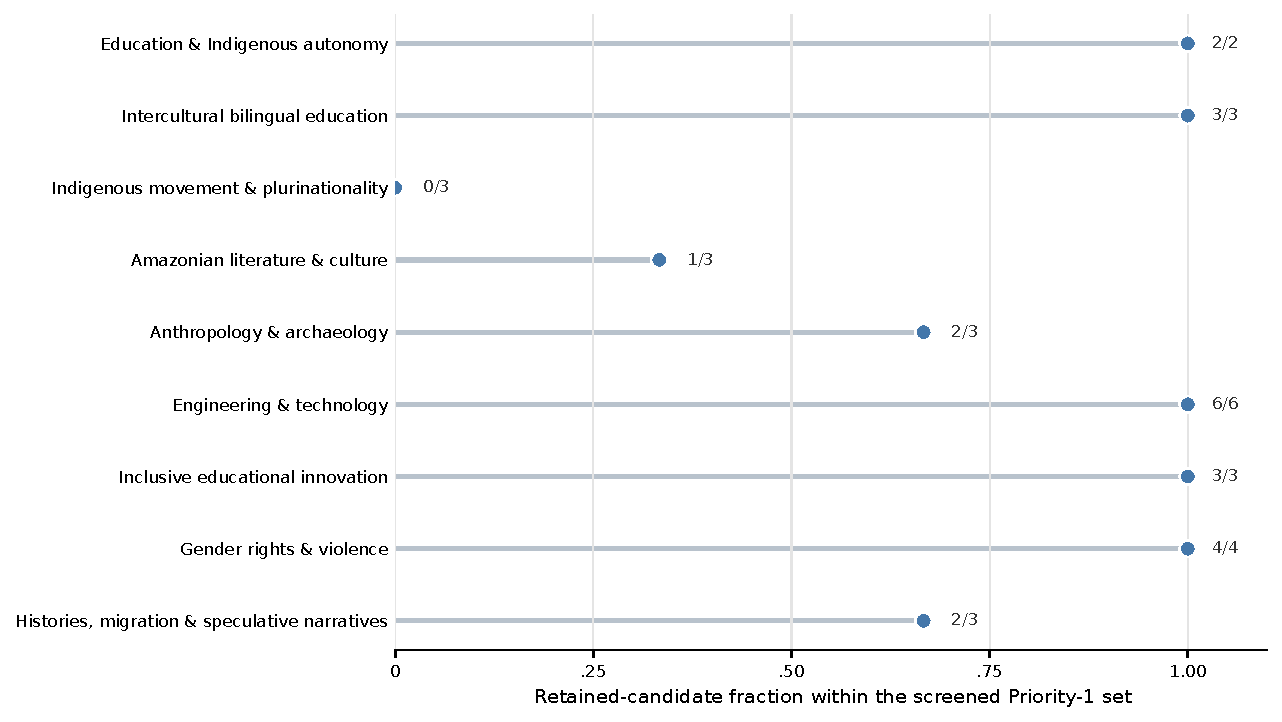
\includegraphics[width=\textwidth]{figures/Fig8_research_fronts.pdf}
\caption{Research Horizon retained-candidate fraction for the nine focal lines after corpus-wide documentary review. Each point gives the retained share within the screened Priority-1 set; adjacent labels report the retained and reviewed counts ($r/n$). Detailed principal, complementary, specific-subline, reserve, and excluded classifications are reported in Table~\ref{tab:rhsummary}.}\label{fig:researchfronts}
\end{figure}

Retention is complete for four focal lines: intercultural bilingual education retains 3/3 candidates, engineering and technology 6/6, inclusive educational innovation 3/3, and gender rights and violence 4/4. Education and Indigenous autonomy also retains both screened candidates (2/2). Anthropology and archaeology and histories/migration each retain 2/3. Amazonian literature and culture retains 1/3. Indigenous movement and plurinationality retains none of its three Priority-1 candidates.

Two cases show why corpus-wide documentary review matters. Indigenous movement and plurinationality had an average preliminary affinity of 91.7/100 across its three candidates, yet two were placed in reserve and one was excluded. Amazonian literature and culture had an even higher preliminary average (94.7) but only one complementary cluster was retained; one candidate remained in reserve and one was excluded. High preliminary affinity therefore does not guarantee that a screened candidate survives documentary review.

\begin{table}[t]
\caption{Research Horizon documentary-review outcomes for the nine focal lines}\label{tab:rhsummary}
\small
\setlength{\tabcolsep}{3pt}
\begin{tabularx}{\textwidth}{@{}Yrrrrrrr@{}}
\toprule
Line & Cand. & Principal & Compl. & Specific & Reserve & Excl. & Retained share \\
\midrule
Education and Indigenous autonomy & 2 & 1 & 1 & 0 & 0 & 0 & 2/2 (1.00) \\
Intercultural bilingual education & 3 & 2 & 1 & 0 & 0 & 0 & 3/3 (1.00) \\
Indigenous movement and plurinationality & 3 & 0 & 0 & 0 & 2 & 1 & 0/3 (0.00) \\
Amazonian literature and culture & 3 & 0 & 1 & 0 & 1 & 1 & 1/3 (0.33) \\
Anthropology and archaeology & 3 & 1 & 0 & 1 & 1 & 0 & 2/3 (0.67) \\
Engineering and technology & 6 & 0 & 0 & 6 & 0 & 0 & 6/6 (1.00) \\
Inclusive educational innovation & 3 & 0 & 1 & 2 & 0 & 0 & 3/3 (1.00) \\
Gender rights and violence & 4 & 2 & 1 & 1 & 0 & 0 & 4/4 (1.00) \\
Histories, migration and speculative narratives & 3 & 1 & 1 & 0 & 0 & 1 & 2/3 (0.67) \\
\bottomrule
\end{tabularx}
\end{table}

These results answer RQ4 only within the screened candidate universe. The retained fraction deliberately exposes candidate-set size instead of converting the outcome into an ordinal category whose attainable ceiling would depend on the number of candidates screened. Because candidate generation is expert-assisted and not exhaustive over the 11,325-topic universe, $H_{\ell}$ is interpreted as the share of screened candidates that survives documentary review. Its denominator is line-specific, and the measure is not calibrated as a global frontier-proximity probability.

\subsection{Cross-layer configurations and answers to the research questions}\label{subsec:integratedresults}

The three evidence layers are compared as a cross-layer configuration while retaining their construct-specific meanings. Figure~\ref{fig:integrated} places the equal-country OpenAlex mapped-topic activity mean on the horizontal axis and the Research Horizon retained-candidate fraction on the vertical axis. Both axes remain on their native descriptive scales, and marker shape identifies the four reference renewals.

\begin{figure}[t]
\centering
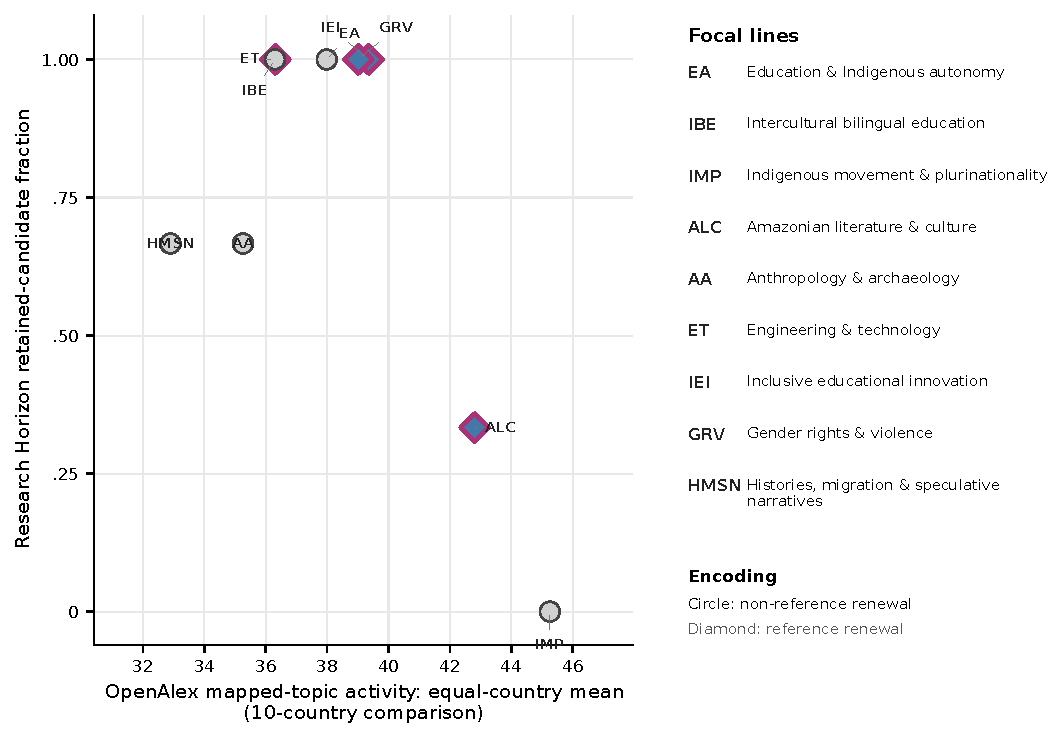
\includegraphics[width=\textwidth]{figures/Fig9_integrated_matrix.pdf}
\caption{Cross-layer configuration of the nine focal editorial lines. The horizontal axis is the equal-country mean of the OpenAlex mapped-topic activity score; the vertical axis is the Research Horizon retained-candidate fraction. Diamonds identify the four reference renewals and circles the remaining focal lines. The axes retain their native descriptive scales, and marker shape identifies reference renewal status.}\label{fig:integrated}
\end{figure}

Three recurring configurations are visible. First, some historically accumulated lines also show relatively high indexed scientific activity, but with different screened-retention patterns. Engineering and technology combines very high internal volume and persistence with the highest United States OpenAlex score and retains all six screened Research Horizon sublines. Anthropology and archaeology has lower internal volume but full persistence, within-family prominence, and retains two of three screened candidates. Education and Indigenous autonomy has the largest internal stock and retains both of its screened candidates.

Second, recent renewal can coexist with a smaller historical stock without implying historical dominance. Intercultural bilingual education, inclusive educational innovation, and gender rights and violence have internal volume scores below 30, satisfy the reference renewal rule, and retain all screened Research Horizon candidates. Their configuration is therefore characterized by a current trajectory and strong survival within the screened frontier set rather than by accumulated catalogue volume.

Third, strong internal specificity can diverge from the selected frontier evidence. Indigenous movement and plurinationality has 92 mapped books, activity in all five decades, and 86.8 continuity, yet its three high-scoring preliminary Research Horizon candidates do not yield a retained research-front match. Amazonian literature and culture satisfies the reference renewal rule and has a strong Brazil-centered OpenAlex profile, but retains only one of three screened Research Horizon candidates. These cases illustrate why internal thematic strength, indexed scientific activity, and screened research-front retention should not be treated as interchangeable measures.

\begin{table}[t]
\caption{Research-question traceability in the proof-of-concept}\label{tab:rqanswers}
\small
\begin{tabularx}{\textwidth}{@{}p{0.08\textwidth}Y Y@{}}
\toprule
RQ & Empirical answer & Main evidence \\
\midrule
RQ1 & The mapped stable semantic core is diverse, persistent, and recently recomposed, while the exact renewal set is partly threshold-sensitive. & 68-topic map; $HHI=0.0259$; ${}^{1}D=51.10$; ${}^{2}D=38.60$; 46 topics active in at least four decades; reference 8-to-4 renewal classification with threshold sensitivity. \\
RQ2 & Expert curation changes a bounded part of the initial algorithmic semantic structure and its effects can be measured explicitly. & 70 initial algorithmic clusters to 68 analytical topics; 389 records with changed topic ID; HHI 0.0316 to 0.0259; effective topics 49.83 to 51.10. \\
RQ3 & Within the bounded ten-country comparison, indexed scientific activity around mapped topics is strongly topic- and territory-specific and remains stable under the tested weighting alternatives. & 90 line-country OpenAlex scores; different leading countries across lines; equal-country vs. 60/40 rank correlation $\rho=0.983$. \\
RQ4 & Within the screened candidate set, retention after documentary review varies sharply across lines and does not follow historical accumulation or preliminary metadata affinity in a simple way. & 23 of 30 Priority-1 clusters retained; retained fractions range from 0/3 to 6/6; movement/plurinationality has high preliminary affinity but no retained research-front match. \\
\bottomrule
\end{tabularx}
\end{table}

Together, the proof-of-concept supports the central methodological proposition of the framework: publisher-level thematic evaluation becomes more interpretable when distinct temporal, structural, geographical, and frontier relations remain visible as separate evidence layers.

\section{Discussion}\label{sec:discussion}

The proof-of-concept supports treating a scholarly publisher as a longitudinal thematic system. Its main empirical contribution is configurational: historical accumulation, recent renewal, database-indexed scientific activity, and research-front retention align for some editorial lines and diverge for others. The discussion therefore focuses on the implications of this longitudinal unit of analysis, the role of documented expert interpretation, and the scope of the two external evidence layers.

\subsection{A publisher catalogue as a longitudinal knowledge structure}

Bibliometric research on books has established the distinctive role of monographs and edited volumes in the social sciences and humanities and has developed publisher prestige surveys, citation indicators, library holdings, and publisher-level assessment approaches \citep{hicks2004four,nederhof2006bibliometric,williams2009monograph,kulczycki2018publication,engels2018books,gimenez2013publishers,white2009libcitations,kousha2011books,torres2014bookcitation,zuccala2015rank}. The present framework centers a complementary object: the thematic organization and temporal development of the catalogue itself.

A catalogue is an ordered historical record shaped by recurring editorial choices, series, collaborations, and changing intellectual agendas. In the \ABYA case, broad long-run persistence coexists with the largest post-prelude compositional shift in the most recent adjacent-window comparison. The coexistence of persistence and recomposition is analytically important because a cross-sectional count cannot represent both properties simultaneously.

This longitudinal view connects publisher analysis to topic-evolution research while changing the unit of interpretation. Dynamic topic models and trajectory methods have mainly followed research fields, venues, papers, or authors over time \citep{blei2006dynamic,schaefermeier2021topicspace,kim2022trajectories}. In a publisher catalogue, the observed trajectory represents editorial accumulation and recomposition. Potential mechanisms include author supply, editorial strategy, co-publishing arrangements, institutional projects, documentary series, and broader scientific change; causal attribution would require additional evidence designed for those mechanisms.

\subsection{Analytical value of multidimensional thematic profiles}

The internal profile represents volume, persistence, continuity, recent growth, and within-family prominence as separate longitudinal properties. This preserves differences among configurations that would otherwise become difficult to interpret. The design is consistent with responsible research-evaluation principles that emphasize contextualized indicators and informed judgment \citep{hicks2015leiden}, and with bibliodiversity research that treats format, language, geography, and infrastructure as distinct dimensions \citep{angioni2026bibliodiversity}.

The two-stage renewal analysis illustrates the same principle at line level. High recent growth can arise from short episodic concentration, whereas a smaller growth ratio can satisfy continuity and recency conditions. The 36-scenario sensitivity grid shows that the exact membership of the reference renewal set is parameter-dependent: Amazonian literature and culture is retained throughout the tested grid, while the other reference lines are less invariant. Future applications should therefore prespecify the renewal thresholds and evaluate their sensitivity within each catalogue.

\subsection{Documented expert curation as an inspectable analytical layer}

Topic-model interpretation benefits from explicit human evaluation because statistical coherence alone does not guarantee substantive interpretability \citep{chang2009tea,mimno2011coherence}. The \ABYA workflow preserves the initial algorithmic state, the curated state, and the document-level differences between them. This provenance makes the magnitude and consequences of expert intervention directly inspectable.

The same separation applies to LLM-assisted labels. GPT-4o proposed topic names from representative titles only after cluster membership had been fixed. Cluster membership, expert structural curation, and post-hoc labeling therefore have distinct provenance, a distinction that is increasingly important in LLM-supported scientometric workflows \citep{lee2026evidence}. The Kipu consolidation provides a concrete editorial example: documentary-series provenance justified a structural correction, and the resulting chronology is interpreted according to catalogue registration dates rather than fine-grained publication timing.

\subsection{External scientific context for the semantic representation}

The OpenAlex layer adds structured scientific context to selected thematic units through topic-country activity across the ten pre-specified countries. Its interpretation is comparative and topic-specific. Direct publisher influence would require linkage evidence such as citations, library use, translations, or other observable relations between \ABYA books and external publications.

This distinction is especially relevant in Latin American social sciences and humanities. OpenAlex can recover broader Spanish-language and SSH output than Scopus in some settings \citep{gallardo2024openalex}, while language metadata and source coverage remain uneven \citep{cespedes2025linguistic,visser2021comparison}. The country profiles should therefore be read as configurations of indexed activity within a bounded database and country universe. The close agreement between equal-country and strategically weighted line summaries shows that the qualitative ordering of focal lines is robust to the tested territorial weighting, while the pre-specified ten-country universe remains part of the study design.

\subsection{Documentary review refines screened research-front retention}

The Research Horizon layer addresses a different construct from OpenAlex indexed activity. Metadata similarity provides an efficient screening mechanism, whereas corpus-wide documentary review determines which selected candidates are retained as principal, complementary, or specific relations. The retained-candidate fraction makes the denominator visible for every focal line and supports a descriptive comparison across the screened set.

The contrast between strong preliminary affinity and subsequent exclusion for some candidates demonstrates the value of documentary review when the analytical claim concerns a substantive relation to the screened research-front candidate. The 11,325-to-73-to-30 audit trail also exposes the selection funnel and preserves reserve and excluded cases. Because screening was expert-assisted and exhaustive recall across all 11,325 topic IDs was outside the design, the resulting fractions characterize the screened Priority-1 candidate set.

\subsection{Contribution of the cross-layer representation}

The cross-layer representation makes visible how historical accumulation, recent renewal, external scientific activity, and retained research-front candidates combine across editorial lines. In representation terms, each focal line retains a semantic identity, hierarchical context, longitudinal profile, and traceable external attributes. For example, a historically large technical line, a smaller renewing educational line, and a historically strong Indigenous-studies line occupy different positions once indexed scientific activity and documentary retention are considered. The analytical value lies in comparing these configurations across distinct dimensions of editorial trajectory and external scientific evidence.

The framework is modular. The internal catalogue layer can support a longitudinal analysis on its own, and the external layers can be added when the research question requires them. Additional indicators can also be incorporated when new metadata are theoretically justified, provided that their construct and provenance remain explicit. This modularity makes the framework suitable for cross-publisher replication while keeping case-specific thresholds and mappings open to prespecification and validation.

\subsection{Limitations}\label{subsec:limitations}

External validity remains to be established beyond the present publisher. The architecture of separated evidence layers, provenance-preserving curation, and longitudinal measures is designed for reuse, while the renewal thresholds, nine focal lines, macro-family cut, ten-country OpenAlex universe, mapping roles, and Research Horizon screening strategy are specific to this case. A second publisher is a direct validation target.

The semantic layer involves two transfers that were not independently validated here. SPECTER2 was developed for scientific-document representation across multiple disciplinary fields \citep{singh2023scirepeval}, whereas this study applies it to a heterogeneous book catalogue. English translations used as model inputs were produced upstream and frozen before the reproducibility package was assembled. Original titles are preserved for the eligible records, but original-language abstracts are not available with comparable completeness. A title-only audit would therefore assess only part of the model input and would not validate the translation of the longer abstracts used for many books. A future replication should audit a stratified title-and-abstract translation sample and compare the reference solution with a multilingual model on original-language inputs.

The reference semantic map covers stable density regions and leaves 1,580 of 3,963 semantically eligible records as HDBSCAN noise. Sensitivity analyses show modest changes in global diversity under complete nearest-centroid forcing ($HHI$ 0.0259 to 0.0242; ${}^{1}D$ 51.10 to 53.01), but a larger change in recent compositional distance (0.363 to 0.258) and an expansion of the reference renewal set from four to ten. A high-confidence reassignment of 166 outliers produces smaller changes and preserves the four reference renewals. Accordingly, the recent recomposition claim refers to the mapped stable semantic core, and exact renewal membership remains sensitive to aggressive outlier treatment. Preserved title-length and duplicate-title diagnostics provide no simple short-text explanation for noise, while complete original-language and series fields are unavailable for a fuller characterization.

Model granularity also depends on clustering choices. A cross-implementation HDBSCAN perturbation on the archived five-dimensional representation reproduces the reference-like $min\_cluster\_size=10$ partition closely (ARI 0.978; NMI 0.985), while values from 8 to 12 change the number of clusters from 92 to 55 and the noise share from 39.7\% to 45.2\%. The archived runtime does not permit an exact historical UMAP $n\_neighbors$ rerun; the reported nearest-neighbor diagnostic in the original 768-dimensional embeddings therefore provides evidence about semantic neighborhood scale rather than UMAP-parameter invariance. Future replication should rerun the full embedding--UMAP--HDBSCAN grid in a single controlled environment.

Expert curation, label revision, OpenAlex role assignment, and Research Horizon final classification were produced by one expert with documented provenance. This supports inspectability, while independent inter-rater reliability remains to be established. Retrospective double coding of the preserved Priority-1 corpora is a legitimate validation design and should be included in subsequent validation work, together with independent coding of a sample of topic labels and OpenAlex mappings.

The external layers are bounded by design and infrastructure. The ten OpenAlex countries form a pre-specified comparison set rather than a global sample. OpenAlex offers useful breadth for Spanish-language and SSH research \citep{gallardo2024openalex}, with remaining metadata and coverage asymmetries \citep{cespedes2025linguistic,visser2021comparison}. Research Horizon is a licensed Clarivate source, and its screened-candidate fractions describe the Priority-1 set rather than exhaustive recall over all 11,325 topic IDs.

The most recent catalogue years are incomplete. Records for 2025 and 2026 reflect the latest catalogue update rather than finalized annual production. Restricting the recent comparison to complete 2022--2024 data increases the 2017--2021 distance slightly from 0.363 to 0.371, supporting the direction of the recent recomposition signal. The Kipu documentary series has an additional chronological constraint because catalogue registration dates are unsuitable for fine-grained publication chronology.

The acquisition layer is only partially traceable at the raw-row exclusion stage. The frozen source metadata records 8,399 rows and 4,142 valid book records but does not preserve a row-level reason for each of the 4,257 exclusions. At least three residual duplicate pairs remain after upstream cleaning. Three known excess records represent at most 0.126\% of the 2,383 mapped books globally; an extreme concentration of all three in a ten-book topic would inflate that topic count by 30\%. Small differences in low-volume topics are therefore interpreted cautiously.

Finally, the renewal rule was formalized retrospectively from the case. The 36-scenario perturbation yields between one and seven retained renewals, with Amazonian literature and culture retained in all tested combinations. Future replications should prespecify the growth-ratio, concentration, recency, 2013 emergence cut, and 2003--2014/2015--2026 comparison windows. The same validation principle applies to expert-defined OpenAlex role weights: Monte Carlo perturbation quantifies weight dependence, while independent role coding would assess interpretive reliability.


\section{Conclusions and future work}\label{sec:conclusion}

This article developed a multidimensional semantic representation framework for reconstructing the long-term thematic trajectory of a scholarly publisher and relating that trajectory to bounded external scientific context. The proof-of-concept combines three analytically distinct layers: the mapped internal thematic structure and its temporal change, OpenAlex-based indexed scientific activity within a bounded country set, and retention of screened Research Horizon candidates after documentary review.

For the \ABYA catalogue, the mapped stable semantic core combines long-term persistence with recent recomposition. Starting from the 70-cluster density-based partition, documented expert curation yields 68 analytical topics through a bounded, document-level traceable intervention. The final map has $HHI=0.0259$, Hill diversity ${}^{1}D=51.10$, and ${}^{2}D=38.60$. The 2017--2021 to 2022--2026 composition differs substantially from the preceding state, and the direction of this shift persists when the recent window is restricted to complete 2022--2024 data and when high-confidence outliers are reassigned. Under the reference two-stage renewal specification, four lines qualify as recent renewal; the sensitivity grid identifies Amazonian literature and culture as the most stable member and shows boundary dependence for the remaining reference lines.

The external layers add complementary information. OpenAlex identifies line-specific geographic configurations of database-indexed scientific activity within the ten pre-specified countries. Research Horizon documentary review retains 23 of 30 Priority-1 candidates, with line-level retained fractions ranging from zero to complete retention. Their joint configuration shows that historical accumulation, recent renewal, indexed scientific activity, and research-front retention can follow different patterns within the same editorial portfolio.

The transferable contribution is the analytical architecture: preservation of initial algorithmic and curated thematic states, explicit interpretive provenance, separate longitudinal measures, and construct-specific connections between the internal map and external scientific infrastructures. The case establishes feasibility and identifies renewal thresholds, focal-line definitions, country universes, hierarchy cuts, and screening procedures as parameters for independent cross-publisher validation.

Future work should proceed through four concrete validation routes. Cross-publisher replication can test the stability and usefulness of the profile dimensions across university, commercial, disciplinary, and multilingual presses. Independent double coding of topic labels, OpenAlex mappings, and preserved Research Horizon corpora can quantify inter-rater agreement. Original-language title-and-abstract corpora can support translation audits and multilingual embedding comparisons. Finally, persistent book identifiers can extend the external layer toward direct evidence of circulation or influence through citations, library holdings, translations, or co-editions.

Taken together, the study establishes the scholarly publisher catalogue as a tractable longitudinal knowledge structure and provides a reproducible semantic representation that preserves explicit thematic units, temporal structure, hierarchical context, and documented interpretive provenance. Bounded external evidence can then be compared with that representation while preserving the distinct scales and meanings of each construct.

\vspace{6pt}

\dataavailability{The original contributions presented in this study are included in the article and in the associated reproducibility materials that can be redistributed. Restrictions apply to raw catalogue text and licensed Research Horizon exports. Further inquiries can be directed to the corresponding author.}

\acknowledgments{Not applicable.}

\conflictsofinterest{\textit{Statement to be finalized by the authors before submission.}}

\abbreviations{Abbreviations}{%
\begin{tabular}{@{}ll}
ARI & Adjusted Rand Index\\
c-TF-IDF & class-based Term Frequency--Inverse Document Frequency\\
EOM & Excess of Mass\\
HDBSCAN & Hierarchical Density-Based Spatial Clustering of Applications with Noise\\
HHI & Herfindahl--Hirschman Index\\
LLM & Large Language Model\\
NMI & Normalized Mutual Information\\
RQ & Research Question\\
SSH & Social Sciences and Humanities\\
UMAP & Uniform Manifold Approximation and Projection
\end{tabular}}

\appendixtitles{yes}
\appendixstart
\appendix

\section{Robustness and sensitivity details}\label{app:robustness}

\subsection{Topic assignment across decades}

Table~\ref{tab:assignment_decades} reports assignment among semantically eligible records. The absence of an abrupt historical collapse does not establish that outliers are missing at random, but it shows that the 39.9\% overall noise share is not generated by one isolated period.

\begin{table}[ht]
\caption{HDBSCAN assignment rate among semantically eligible books by decade}\label{tab:assignment_decades}
\small
\begin{tabular}{lrrr}
\toprule
Period & Eligible & Assigned & Assignment rate \\
\midrule
1978--1989 & 164 & 107 & 65.2\% \\
1990--1999 & 781 & 500 & 64.0\% \\
2000--2009 & 954 & 570 & 59.7\% \\
2010--2019 & 1,515 & 881 & 58.2\% \\
2020--2026 & 549 & 325 & 59.2\% \\
\bottomrule
\end{tabular}
\end{table}

\subsection{Hierarchical family cut}

The number of macro-families changes monotonically around the selected hierarchy threshold, with a short plateau at nine families (Table~\ref{tab:family_sens}). This is why the family layer is interpreted as a useful mesoscale organization rather than a uniquely identified taxonomy.

\begin{table}[ht]
\caption{Sensitivity of macro-family count to the hierarchical cut}\label{tab:family_sens}
\small
\begin{tabular}{rrrrrrrr}
\toprule
Cut threshold & 4.00 & 4.25 & 4.50 & 4.75 & 5.00 & 5.25 & 5.50 \\
\midrule
Macro-families & 12 & 11 & 10 & 9 & 9 & 8 & 7 \\
\bottomrule
\end{tabular}
\end{table}

\subsection{Outlier-reassignment stress tests}

The reference solution leaves HDBSCAN noise unassigned. Table~\ref{tab:outlier_sens} compares that state with two deliberately different reassignment scenarios. The high-confidence scenario assigns 166 noise records whose centroid similarity and assignment margin both exceed 25th-percentile thresholds derived from assigned records; complete forcing assigns all 1,580 noise records to the nearest final-topic cosine centroid. The controlled scenario leaves global diversity and the four reference renewals unchanged. Complete forcing retains those four lines but adds six further renewals, while also reducing the recent compositional distance. This contrast shows that line-level temporal classification is more sensitive than overall diversity to aggressive outlier treatment.

\begin{table}[ht]
\caption{Sensitivity of global diversity, recent compositional change, and renewal membership to outlier reassignment}\label{tab:outlier_sens}
\small
\setlength{\tabcolsep}{3pt}
\begin{tabularx}{\textwidth}{@{}Yrrrrrr@{}}
\toprule
Scenario & Mapped & $HHI$ & ${}^{1}D$ & ${}^{2}D$ & Recent distance & Renewals \\
\midrule
Reference stable core & 2,383 & 0.0259 & 51.10 & 38.60 & 0.363 & 4 \\
High-confidence reassignment & 2,549 & 0.0256 & 51.34 & 39.08 & 0.334 & 4 \\
All noise forced to nearest centroid & 3,963 & 0.0242 & 53.01 & 41.33 & 0.258 & 10 \\
\bottomrule
\end{tabularx}
\end{table}

In the complete-forcing scenario, all four reference renewals remain selected and six additional topics enter the renewal set. The robustness result is therefore asymmetric: the reference lines are not lost, but the specificity of the four-line classification depends on preserving diffuse observations as noise rather than forcing complete coverage.

\subsection{Renewal-threshold perturbation}

The reference two-stage renewal specification is evaluated for threshold sensitivity. Across 36 combinations of growth-ratio, episodicity, and final-year thresholds, the number of retained renewals varies from one to seven. Table~\ref{tab:renewal_survival} reports selection frequencies for every topic retained in at least one perturbation. Amazonian literature and culture is the only line retained under all tested combinations.

\begin{table}[ht]
\caption{Selection frequency under 36 renewal-threshold combinations}\label{tab:renewal_survival}
\small
\begin{tabularx}{\textwidth}{@{}Yr@{}}
\toprule
Topic & Share of scenarios retained \\
\midrule
Amazonian literature and culture & 100.0\% \\
Inclusive educational innovation & 75.0\% \\
Gender rights and violence & 66.7\% \\
Intercultural bilingual education & 66.7\% \\
Interculturality and cultural educational management & 33.3\% \\
Anthropology and material relations & 33.3\% \\
Digital media and social networks & 25.0\% \\
\bottomrule
\end{tabularx}
\end{table}

\subsection{Recent-window completeness}

The largest recent reference distance is not inflated by the incomplete 2025--2026 tail. The distance from 2017--2021 to 2022--2026 is 0.363, whereas replacing the second period with complete 2022--2024 data yields 0.371. Under the high-confidence outlier scenario the corresponding values are 0.334 and 0.341. The recent recomposition signal therefore persists when incomplete end years are excluded.

\subsection{Clustering-granularity diagnostics}

A cross-implementation HDBSCAN perturbation was run on the archived five-dimensional UMAP representation. The reference-like setting ($min\_cluster\_size=10$ with the adjusted scikit-learn $min\_samples$ semantics) closely matches the frozen initial algorithmic solution (ARI 0.978; NMI 0.985). Moving the minimum cluster size from 8 to 12 changes the number of clusters from 92 to 55 and the noise share from 39.7\% to 45.2\% (Table~\ref{tab:hdbsens}). These values demonstrate expected granularity dependence rather than a uniquely determined cluster count.

\begin{table}[ht]
\caption{Cross-implementation HDBSCAN minimum-cluster-size sensitivity}\label{tab:hdbsens}
\small
\begin{tabular}{rrrrr}
\toprule
Minimum cluster size & Clusters & Noise share & ARI vs. frozen & NMI vs. frozen \\
\midrule
8  & 92 & 0.397 & 0.706 & 0.851 \\
9  & 84 & 0.414 & 0.767 & 0.881 \\
10 & 70 & 0.402 & 0.978 & 0.985 \\
11 & 62 & 0.424 & 0.837 & 0.903 \\
12 & 55 & 0.452 & 0.740 & 0.855 \\
\bottomrule
\end{tabular}
\end{table}

An exact historical UMAP $n\_neighbors$ rerun was not reconstructed from the archived runtime. As a narrower diagnostic, the mean share of same-topic neighbors in the original 768-dimensional SPECTER2 space decreases from 0.748 at $k=10$ to 0.673 at $k=15$, 0.614 at $k=20$, and 0.528 at $k=30$. This indicates that the final topics retain substantial local semantic coherence near the reference neighborhood scale, but it should not be read as a direct UMAP-parameter sensitivity experiment.

\subsection{Characterization of unassigned records and duplicate bound}

Within the preserved analytical state, unassigned records have a median original-title length of 66 characters compared with 60 for assigned records; median model-text lengths are 64 and 59, respectively. Exact duplicate-title shares are 12.9\% and 12.5\%. These diagnostics do not support a simple ``short text produces noise'' explanation. Complete original-language and series metadata are not preserved at sufficient resolution to test all other mechanisms that could plausibly contribute to non-assignment.

At least three residual duplicate pairs are known after upstream cleaning. If each pair contributes one excess record, the maximum known global inflation is three records, or 0.126\% of the 2,383 mapped books. An extreme local upper bound occurs if all three excess records belong to a smallest ten-book topic, in which case that topic's count could be inflated by 30\%. This worst case is not observed evidence about the duplicate locations; it is reported only to bound the possible effect of the known minimum duplicate count.

\subsection{OpenAlex territorial scenario}

A pre-specified strategic territorial scenario assigns 60\% of the line-level weight to Ecuador, Mexico, and Spain and 40\% to the other seven countries. The equal-country mean serves as the scientific reference, while the 60/40 weighting is retained as an alternative strategic scenario. Table~\ref{tab:oa_sens} compares the equal-country mean with the strategic scenario. The ordering is highly similar ($\rho=0.983$), but the differences are retained to prevent the strategic weighting from being mistaken for an objective ranking.

\begin{table}[ht]
\caption{Equal-country and strategic OpenAlex line summaries}\label{tab:oa_sens}
\small
\begin{tabularx}{\textwidth}{@{}Yrrr@{}}
\toprule
Line & Equal-country mean & 60/40 scenario & Difference \\
\midrule
Indigenous movement and plurinationality & 45.26 & 46.45 & +1.19 \\
Amazonian literature and culture & 42.81 & 43.00 & +0.20 \\
Inclusive educational innovation & 39.36 & 42.57 & +3.21 \\
Gender rights and violence & 39.02 & 39.73 & +0.71 \\
Education and Indigenous autonomy & 37.99 & 38.96 & +0.98 \\
Intercultural bilingual education & 36.31 & 36.32 & +0.01 \\
Engineering and technology & 36.30 & 36.79 & +0.49 \\
Anthropology and archaeology & 35.26 & 34.89 & -0.36 \\
Histories, migration and speculative narratives & 32.90 & 33.07 & +0.18 \\
\bottomrule
\end{tabularx}
\end{table}

\subsection{OpenAlex weight perturbation}

To assess whether the geographic pattern depends on the exact component and mapping-role weights, we independently perturbed the five topic-country component weights and the four mapping-role weights by $\pm25\%$ in 5,000 Monte Carlo simulations. Each simulation was renormalized to the same 0--100 line-country scale. The aggregate country ordering was highly stable: the United States ranked first in all simulations, while Spain and Brazil remained in the top three in all simulations. At line level, the leading country was unchanged in all simulations for six lines and in at least 99.5\% for two additional lines. Amazonian literature and culture was the most weight-sensitive case: Brazil remained the leading country in 70.0\% of simulations, followed by the United States (17.2\%) and Spain (12.8\%). This sensitivity is reported as a property of that line rather than suppressed by the aggregate ranking.

\begin{table}[ht]
\caption{Monte Carlo stability of selected OpenAlex geographic conclusions (5,000 simulations)}\label{tab:oa_mc}
\small
\begin{tabularx}{\textwidth}{@{}Ylr@{}}
\toprule
Quantity & Modal outcome & Stability \\
\midrule
Aggregate country rank 1 & United States & 100.0\% \\
Aggregate countries in top 3 & United States, Spain, Brazil & 100.0\% each \\
Movement/plurinationality line leader & Argentina & 99.6\% \\
Anthropology/archaeology line leader & United States & 99.7\% \\
Amazonian literature/culture line leader & Brazil & 70.0\% \\
\bottomrule
\end{tabularx}
\end{table}

\begin{adjustwidth}{-\extralength}{0cm}
\reftitle{References}
\bibliography{references}
\end{adjustwidth}
\PublishersNote{}
\end{document}
